%======================================================================
% ScholarPath AdDU -- Capstone Manuscript (Master Driver File)
% ----------------------------------------------------------------------
% Preamble discipline: global settings only. All body content lives in
% chapters/*.tex and is wired in below via \input. Do not add prose here.
%======================================================================
\documentclass[12pt,letterpaper]{report}

%----- Encoding, fonts, and page geometry -----------------------------
\usepackage[T1]{fontenc}
\usepackage[utf8]{inputenc}
\usepackage{lmodern}   % scalable fonts required by microtype font expansion
\usepackage[letterpaper,margin=1in]{geometry}
\usepackage{microtype}

%----- Mathematics -----------------------------------------------------
\usepackage{amsmath}
\usepackage{amssymb}

%----- Graphics, tables, and listings ----------------------------------
\usepackage{graphicx}
\graphicspath{{figures/}}
\usepackage{booktabs}
\usepackage{longtable}
\usepackage{array}
\usepackage{enumitem}
\usepackage{xurl}     % allow URL line breaks anywhere (used in Appendix A)
\usepackage{listings}
\lstset{
  basicstyle=\ttfamily\small,
  breaklines=true,
  frame=single,
  framesep=6pt,
  aboveskip=12pt,
  belowskip=12pt,
  captionpos=b,
  keywordstyle=\bfseries,
  commentstyle=\itshape\color{black!60},
  showstringspaces=false
}

%----- Bibliography ----------------------------------------------------
\usepackage{csquotes}
\usepackage[backend=biber,style=numeric-comp,sorting=none,maxbibnames=99]{biblatex}
\addbibresource{references.bib}

%----- Hyperref (load last) --------------------------------------------
\usepackage[hidelinks]{hyperref}

%======================================================================
% Document metadata
%======================================================================
\title{%
  {\LARGE\bfseries ScholarPath AdDU: A Web-Based Scholarship Application\\[4pt]
  Processing and Committee Decision-Support System\\[4pt]
  for Ateneo de Davao University's Internal Scholarship Tracks\par}
  \vspace{18pt}
  {\large A Research Project Presented to the Faculty of the\\
  Computer Studies Cluster, School of Arts and Science\\
  Ateneo de Davao University, Davao City\par}
  \vspace{18pt}
  {\normalsize In Partial Fulfillment of the Requirements in\\
  Capstone Project and Research 1, 2nd Semester, SY 2025--2026\par}
}
\author{%
  Operario, Raphael Miguel\\
  Belen, Brendon Justine\\
  Espinosa, Eriel John\\[10pt]
  \normalsize Adviser: Adrian Ablazo, MSc.
}
\date{April 2026}

%======================================================================
% Front matter
%======================================================================
\begin{document}

\begin{titlepage}
  \centering
  \vspace*{1cm}
  
\includegraphics[width=0.22\textwidth]{addu_logo.png}\par
  \vspace{1.5cm}
  {\LARGE\bfseries ScholarPath AdDU: A Web-Based Scholarship Application Processing and Committee Decision-Support System for Ateneo de Davao University's Internal Scholarship Tracks\par}
  \vspace{1.5cm}
  {\large A Research Project Presented to the Faculty of the Computer Studies Cluster, School of Arts and Science\\ Ateneo de Davao University, Davao City\par}
  \vspace{1cm}
  {\normalsize In Partial Fulfillment of the Requirements in Capstone Project and Research 1, 2nd Semester, SY 2025--2026\par}
  \vspace{1.5cm}
  {\large
    Raphael Miguel Operario\\
    Brendon Justine Belen\\
    Eriel John Espinosa\par}
  \vspace{1cm}
  {\normalsize Adviser: Adrian Ablazo, MSc.\par}
  \vfill
  {\normalsize April 2026\par}
\end{titlepage}

\tableofcontents
\clearpage

%======================================================================
% Body -- one \input per chapter (preamble discipline: no prose here)
%======================================================================
\chapter{Introduction}
\label{ch:introduction}

\section{Background of the Study}
\label{sec:background}

Globally, universities are transitioning from traditional, paper-based administrative workflows to digital ecosystems to enhance student access to educational funding. This digitalization is increasingly necessary due to rising educational costs and expanding student populations. In the Philippines, the steady growth of the higher education sector \cite{ref29} has coincided with tuition fee increases across numerous private institutions, driven by inflation and operational adjustments \cite{ref11,ref19}. While financial aid is available through state-sponsored grants \cite{ref21,ref44}, international educational investments \cite{ref45}, and private corporate foundations \cite{ref1,ref40}, the institutions that administer this aid must still collect, verify, and deliberate on large volumes of applicant documents. At Ateneo de Davao University (AdDU), students face similar financial pressures, exacerbated by recent and proposed tuition increases. AdDU's wider financial aid landscape spans internally funded endowments, external corporate partnerships, and state-sponsored grants \cite{ref2,ref8} (Appendix~\ref{app:pipelines}). Within that landscape, the university itself selects scholars through three internal tracks, which together receive approximately 1,326 applicants per cycle (Table~\ref{tab:tracks}). External and government grants fall outside the university's selection process; AdDU only processes their disbursement after receiving each grantor's official beneficiary roster.

% TODO(OPEN-5): currency and period of the income limit; unit of the minimum GIA grant.
% TODO(OPEN-3), TODO(OPEN-9): Jubilee guarantee vs. program minimums; SOP "academic grant" = Jubilee?
\begin{table}[htbp]
  \centering
  \small
  \caption{Internal Scholarship Tracks Governed by ScholarPath AdDU}
  \label{tab:tracks}
  \begin{tabular}{@{}p{2.3cm}p{3.6cm}p{3.6cm}p{4.9cm}@{}}
    \toprule
    Track & Beneficiaries & Grant & Key Rules \\
    \midrule
    Jubilee Scholarship & Certified high school Rank~1 and Rank~2 graduates & Fixed: Rank~1 (Valedictorian) 100\% tuition; Rank~2 (Salutatorian) 50\% tuition & Requires an official ranking certificate; rates are fixed; program-specific admission minimums are applied by each school \\
    Grant-in-Aid (GIA) & Financially challenged students below the university's household income ceiling & Variable, up to 100\% tuition & Requires verified income documents (BIR Form 2316 or sworn statement); slots are highly competitive \\
    Working Scholars & Need-based applicants willing to render service & 100\% tuition, fulfilled through assigned campus work hours instead of cash & Same initial screening as GIA; work obligations are tracked in the Academic Trajectory Path \\
    \bottomrule
  \end{tabular}
\end{table}

Admission to these tracks follows the university's Standard Procedure for Scholarship Applications (SOP) \cite{ref51}, an eight-step process that runs from the application announcement through document submission, verification, interview, deliberation by the School Scholarship Subcommittee, and the release of results by the Office of Admission. Two features of this process create persistent operational strain. First, document collection is single-phase and paper-heavy: every applicant submits a complete physical file, and an application with a missing or illegible document can be rejected outright. Second, final selection belongs to five School Scholarship Subcommittees, those of the School of Nursing (SON), the School of Engineering and Architecture (SEA), the School of Business and Governance (SBG), the School of Education (SOE), and the School of Arts and Sciences (SAS). Each subcommittee applies its own selection criteria, so applicant data must be collated manually for each school.

To address this, this project proposes ScholarPath AdDU, a Data-Feeding Committee Portal for AdDU's internal scholarship admission process. The platform is deliberately not an automated matching tool. It structures, verifies, and presents applicant data to the people who decide, and it records every decision that changes an applicant's status together with the person who made it. The name ScholarPath refers to two structured paths: the Application Lifecycle Path, which carries an applicant from registration to an award, waitlist, or disapproval outcome, and the Academic Trajectory Path, which tracks an awarded scholar's academic standing, service obligations, and graduation. The platform's first core component is a two-stage digital submission into a Document Vault backed by Supabase Storage. Phase~1 Pre-qualification collects the documents needed to screen basic eligibility, and Phase~2 Full Verification collects the remaining documents for review by the University Scholarship Office. The second component is the Conditional Revert protocol, which gives every incomplete file five calendar days to be corrected before a staff member decides its outcome. The third component is committee-side filtering that partitions applicants by school and presents each subcommittee's data under that school's criteria. The fourth is an event-driven notification subsystem that delivers SMS and email alerts via Twilio and SendGrid for submission deadlines, correction requests, and results released by the Office of Admission.

\section{Problem Statement}
\label{sec:problem}

Ateneo de Davao University (AdDU) lacks a digital system to manage the admission process of its internal scholarship tracks. The current reliance on a paper-based procedure creates systemic strain on applicants and on the offices and committees that evaluate them. Specifically, the current process presents the following problems:

\begin{enumerate}
  \item Single-Phase, Paper-Heavy Document Collection: Applicants must assemble and physically submit a complete file at once. A missing or illegible document can lead to an abrupt rejection, with no structured window for correction.
  \item Fragmented Committee Data and Untraceable Decisions: Five School Scholarship Subcommittees apply different selection criteria to approximately 1,326 applicants per cycle, and their data must be collated manually. Decisions are not recorded in a form that traces each status change to the person who made it.
  \item Status and Deadline Communication Deficits: The absence of proactive status updates and deadline reminders leaves applicants unaware of submission windows and correction requests, leading to missed deadlines and incomplete files.
\end{enumerate}

Consequently, this study seeks to answer the following specific research questions:

\begin{enumerate}
  \item What is the perceived reduction in the time and effort AdDU scholarship applicants spend on the application process when using the two-stage digital submission of ScholarPath AdDU compared to the current paper-based process?
  \item How does the ScholarPath AdDU Application Lifecycle workflow perform in terms of (a) functional correctness, specifically whether status transitions, including Conditional Revert and Lapsed, match the expected outputs of a structured Lifecycle Test Case Matrix with no status change lacking a recorded human actor, and (b) perceived usefulness of the Data-Feeding Committee Portal to University Scholarship Office staff and School Scholarship Subcommittee members?
  \item To what extent does the automated notification subsystem reduce missed submission deadlines and uncorrected incomplete files among applicants?
  \item What is the overall system usability and performance efficiency of ScholarPath AdDU as evaluated by users based on the ISO/IEC 25010 functional suitability standards?
\end{enumerate}

\section{Objectives of the Study}
\label{sec:objectives}

General Objective: To design, develop, and evaluate ScholarPath AdDU, a data-feeding scholarship application lifecycle and committee decision-support system for Ateneo de Davao University. The platform aims to replace the paper-based scholarship admission process with a digital workflow that supports, but never replaces, the people who decide.

Specific Objectives:

\begin{enumerate}
  \item To develop a Data-Feeding Committee Portal that partitions applications by school, presents each School Scholarship Subcommittee's data under that school's rule set, and records every status change in an audit log with the acting user and timestamp, such that no module assigns, approves, or disapproves an applicant without a recorded human action.
  \item To implement a two-stage digital submission, consisting of Phase~1 Pre-qualification and Phase~2 Full Verification, into a Document Vault verified entirely within the University Scholarship Office, together with a five-day Conditional Revert protocol for incomplete files.
  \item To implement a proactive notification system that alerts applicants to submission deadlines, correction requests, and released results through automated, event-driven SMS and email delivery.
  \item To administer a Pre-Study Student Problem Validation Survey among current or recent AdDU scholarship applicants to establish baseline data on the perceived time and effort burden of the existing process, and to administer a Post-Prototype Perceived Effort Survey to the same cohort following prototype testing, enabling a direct comparative analysis for Research Questions 1 and 3.
  \item To evaluate the ScholarPath AdDU functional prototype using a task-based usability testing protocol aligned with ISO/IEC 25010 standards, measuring functional suitability, performance efficiency, and system usability via the System Usability Scale (SUS).
\end{enumerate}

\section{Significance of the Study}
\label{sec:significance}

The implementation of ScholarPath AdDU provides practical, structural benefits to key stakeholders within the university. For applicants, the system replaces a single physical submission with a two-stage digital process and gives them a defined window to correct incomplete files instead of facing abrupt rejection. For the University Scholarship Office, the platform digitizes document verification and application tracking, reducing the operational burden of handling approximately 1,326 physical files per cycle. For the five School Scholarship Subcommittees, the platform delivers each school's applicant data already partitioned and filterable under that school's criteria, while leaving every selection decision with the committee. For the Office of Admission, the platform records the handoff of each accepted list and ties applicant notifications to its release of results. Because every status change is logged with the responsible person, the system also supports the traceability expected in institutional quality audits. Additionally, this study contributes to the broader field of higher education management by documenting an architectural framework for migrating scholarship admission from paper to a digital, human-governed workflow under the constraints of national data privacy legislation.

\section{Scope and Limitations}
\label{sec:scope}

This study is bounded by the design, development, and evaluation of a functional web and mobile application prototype for Ateneo de Davao University. The platform's scope is defined by its target users, the scholarship tracks it governs, and the specific administrative functions it digitizes. It does not extend to actual monetary disbursement, integration with the university's finance ledger, or selection for external scholarships. Within these boundaries, the system addresses the digital lifecycle of internal scholarship admission, from applicant registration and two-stage document submission through verification, interview scoring, committee selection, the release of results, and the Academic Trajectory Path of awarded scholars.

Scope. The system scope includes:

\begin{itemize}
  \item Target Audience Coverage: The platform is designed for applicants to AdDU's internal scholarship tracks, awarded scholars, University Scholarship Office staff, interview panels, the five School Scholarship Subcommittees, and the Office of Admission.
  \item Scholarship Coverage: The platform governs the three internal scholarship tracks: the Jubilee Scholarship, Grant-in-Aid (GIA), and Working Scholars. External and government grants are recorded only as a non-selection pathway for disbursement.
  \item Core Functionality:
  \begin{itemize}
    \item A Data-Feeding Committee Portal that partitions applications by school, applies each school's rule set as screening flags and sort orders, and records every human decision in an audit log.
    \item A Document Vault receiving a two-stage digital submission (Phase~1 Pre-qualification and Phase~2 Full Verification), with verification performed entirely within the University Scholarship Office.
    \item A Conditional Revert protocol that gives incomplete files five calendar days for correction, after which a staff member confirms any disapproval.
    \item An automated notification subsystem delivering deadline reminders, correction notices, and released results via SMS and email.
    \item Scholar movement support for inter-track realignment, external grant program transfer, and waitlist reallocation, each confirmed by a person.
  \end{itemize}
  \item Development Approach: The prototype implements a hybrid mobile and web architecture to ensure cross-platform compatibility. The system uses standard web frameworks and cloud-based databases to manage real-time synchronization, cloud storage, and secure user authentication.
  \item Evaluation Scope: Usability testing based on ISO/IEC 25010 standards will involve a purposive sample of approximately 10 to 15 participants drawn from current or recent scholarship applicants, University Scholarship Office staff, and School Scholarship Subcommittee members. The evaluation will use a mixed-method approach, combining task-based observational testing (measuring completion rates and time-on-task) with post-session instruments: the System Usability Scale (SUS), the Post-Prototype Perceived Effort Survey (Appendix~\ref{app:post-survey}) compared against the pre-study baseline (Appendix~\ref{app:pre-survey}), and the Committee Portal Usefulness Survey (Appendix~\ref{app:committee-survey}). Functional correctness will be evaluated separately through a Lifecycle Test Case Matrix.
\end{itemize}

Limitations. This study acknowledges the following realistic constraints that define its boundaries:

\begin{itemize}
  \item Decision-Support Only: The platform structures, filters, and presents applicant data. It does not select, award, approve, or disapprove any applicant. Screening flags and school rule sets inform the University Scholarship Office and the School Scholarship Subcommittees, which retain exclusive authority over every status decision.
  \item Financial Transaction Limitation: The prototype does not handle actual monetary disbursements, bank routing, or direct tuition fee deductions from the university's finance ledger.
  \item External Grant Limitation: External and government grants, such as DOST, local government unit, and private foundation scholarships, are outside the platform's selection process. The platform does not grant external organizations access to the AdDU database, and applicants must still complete any external application through the grantor's own channels.
  \item Manual Verification of Academic Records: The platform does not integrate with the records of the applicant's high school or with the AdDU entrance examination system. The high school general average and entrance exam result are read from uploaded documents and verified manually by University Scholarship Office staff; the accuracy of screening flags therefore depends on that verification.
  \item No Algorithmic Selection: The platform does not implement any algorithm for determining which among multiple qualified applicants should receive a scholarship when applicants exceed the available slots. Sorting and filtering follow criteria set by each subcommittee, and the final selection, including any ranking among equally qualified applicants, remains with the School Scholarship Subcommittee.
  \item User Base Limitation: System access is restricted to applicants to AdDU's internal college scholarship tracks, awarded scholars, and designated university personnel. Basic education units, Graduate School students, and the general public are excluded from this platform.
  \item Testing Scope Limitation: Usability evaluation involves a purposive sample of participants rather than a university-wide deployment. Findings will inform prototype refinement for the capstone requirements but do not constitute definitive statistical claims about the system's efficacy across the entire AdDU population.
  \item Prototype-Based Time Estimation Constraint: The participant time estimates collected through the Post-Prototype Perceived Effort Survey (Appendix~\ref{app:post-survey}) are based on a single, controlled prototype testing session rather than sustained real-world use of the deployed system. Consequently, these estimates may not fully reflect actual time-on-process in practice, as factors such as varying network conditions, individual document readiness, and accumulated platform familiarity over repeated use could produce meaningfully different results from those observed during the evaluation session.
  \item Unconfirmed Procedural Parameters: Several procedural details, including interview panel composition, the starting event of the five-day correction window, and the precedence between the Jubilee grant and program-specific admission minimums, remain under confirmation with the University Scholarship Office. The platform implements these as configurable settings rather than fixed rules.
\end{itemize}

\chapter{Review of Related Works}
\label{ch:rrl}

\section{Digital Transformation in Higher Education Administration}
\label{sec:digital-transformation}

The transition from traditional administrative processes to digital ecosystems is a critical focus for modern educational institutions. Early Management Information Systems (MIS) successfully digitized basic student records but frequently functioned as siloed databases that failed to integrate cross-departmental workflows \cite{ref3,ref5}. This fragmentation resulted in underutilized resources, compromised administrative efficiency, and unequal educational access, not merely because paper was replaced by screens, but because the underlying workflows remained disconnected. Institutions globally have recognized that streamlining student services requires unified digital workflows as a structural prerequisite for operational sustainability \cite{ref46}. Contemporary digital transformation therefore requires interoperable architectures: systems capable of unifying data collection, processing, and reporting across departments into a single, coherent workflow \cite{ref36}. Kayanja et al. \cite{ref46} confirm in their 2025 study of fully automated and paperless systems in higher education that the most significant efficiency gains emerge not from digitizing isolated records, but from architecturally integrating those records into cross-departmental process flows. This finding is directly applicable to scholarship administration, where document submission, verification, interview scoring, and committee deliberation currently exist as separate, disconnected processes at most Philippine higher education institutions. At AdDU, these steps span the University Scholarship Office, interview panels, five School Scholarship Subcommittees, and the Office of Admission. The literature therefore establishes that the effectiveness of digital transformation in higher education depends on interoperable, cross-departmental architectures, the foundational design principle motivating ScholarPath AdDU's centralized, Supabase-backed infrastructure.

\section{Web-Based Scholarship Management Systems}
\label{sec:web-systems}

While web technologies are increasingly leveraged for scholarship management globally, the literature focusing on Southeast Asian and Philippine higher education contexts reveals both what existing systems achieve and where they fall short. Bagaporo and Espinosa \cite{ref12} developed an Online Scholarship Management System for Camarines Sur Polytechnic Colleges (CSPC), implementing a centralized digital repository that consolidates scholarship listings, automates announcement dissemination to enrolled students, and provides an administrative dashboard for monitoring scholarship status. The system successfully eliminated the need for physical bulletin boards and improved information reach across the multi-campus institution. However, the platform stops at information dissemination: document submission remained a manual, offline process, and students were still required to process physical paperwork and submit it to the respective offices in person \cite{ref12}.

Daluyon and Bilog \cite{ref14} developed a Scholarship Management Information System specifically for State Universities and Colleges (SUCs) in Rizal, incorporating online application submission and a structured administrative review interface. Their system advanced beyond the CSPC implementation by digitizing the submission process, reducing paper routing, and enabling administrators to view and sort applications from a centralized dashboard. Crucially, however, Bilog's evaluation found that unaided self-assessment of eligibility was the primary driver of application errors and administrative rework across multi-campus deployments. Students frequently submitted applications for grants they did not qualify for, generating review bottlenecks for administrative staff \cite{ref14}. This finding motivates ScholarPath AdDU's Phase~1 Pre-qualification, in which the platform flags baseline criteria early and a University Scholarship Office staff member confirms the outcome, rather than leaving applicants to judge their own eligibility or letting software decide it.

Al-Ayyubi and Maulana \cite{ref3} designed a web-based scholarship management information system for a higher education institution in Indonesia, achieving efficient dissemination of scholarship information and basic application form routing through a unified web interface. The system demonstrated measurable improvements in processing speed and information accessibility. Yet the researchers themselves identified the architectural absence of integrated, secure document handling as a critical and recurring gap: applicants entered details through forms, but prerequisite documents such as transcripts and income proofs were still submitted physically and managed separately \cite{ref3}. This gap informs the Document Vault architecture in ScholarPath AdDU, which receives documents in two submission phases and supports correction within the platform.

At the international level, Amer \cite{ref5} at the Lebanese American University developed a Smart Scholarship Management System as an all-in-one solution, integrating application submission, document handling, and status tracking into a unified platform. The system demonstrated the technical feasibility of end-to-end digital scholarship administration but was built for a single decision-making body applying one set of criteria. The challenge of serving several academic units that each apply their own selection rules to a shared applicant pool was not a design constraint of that system. The reviewed literature therefore reveals a clear progression in capability: from static digital repositories \cite{ref12}, to submission-enabled portals \cite{ref14,ref3}, to integrated multi-function platforms \cite{ref5}. None demonstrates a validated solution that combines phased digital document submission, structured correction of incomplete files, and decision support for multiple school-level committees whose every decision is recorded, the combination that ScholarPath AdDU addresses.

\section{Automated Decision-Making versus Decision Support in Scholarship Selection}
\label{sec:decision-support}

In digital scholarship systems, the technical mechanism by which applicants are evaluated against eligibility criteria varies substantially across the reviewed literature, and these differences in mechanism determine both the quality of outcomes and who is accountable for them. Three dominant implementation patterns emerge: keyword-overlap matching, threshold-based sequential rule evaluation, and machine-learning-driven classification, each carrying distinct computational behaviors and institutional tradeoffs. Keyword-overlap matching operates by tokenizing profile fields and tallying term coincidences against grant descriptions. Systems relying solely on this mechanism are computationally incapable of evaluating intersecting numerical constraints as a unified logical gate. Orgianus et al. \cite{ref36} document this explicitly: keyword-based retrieval produced persistent false-positive matches because a keyword engine performs term frequency comparisons, not constraint satisfaction. Threshold-based sequential rule evaluation, as implemented by Bilog \cite{ref14}, advances beyond keyword matching by encoding eligibility criteria as conditional logic, but evaluates constraints independently and without formal priority ordering, producing conflict resolution failures at edge cases that Section~\ref{sec:screening-deployed} examines in detail. A third pattern, machine-learning classification, is documented by Kanwal et al. \cite{ref50}, whose C4.5 decision tree achieved 95.62\% prediction accuracy on scholarship eligibility data. However, ML-derived decision boundaries carry two institutional liabilities: the model requires retraining whenever criteria change, and its decisions offer no interpretable audit trail, a concern for accountability and for compliance under RA 10173 that the authors themselves acknowledge \cite{ref50}.

These findings establish a hierarchy of tradeoffs: keyword matching fails at constraint evaluation; sequential rule evaluation fails at conflict resolution; ML classification fails at interpretability and update responsiveness. A common thread runs through all three. Each pattern places the eligibility or selection decision inside the software, and each failure mode therefore becomes a wrong decision made without a responsible person. ScholarPath AdDU draws the opposite conclusion from the same evidence. Its rules encode baseline and school-specific criteria as screening flags and sort orders, but the decision that changes an applicant's status is always made and recorded by a University Scholarship Office staff member, an interview panel, or a School Scholarship Subcommittee. This design is consistent with the institutional directive, arising from AdDU's preparation for a quality audit, that no algorithm selects scholars \cite{ref52}. % TODO(L-6): add team-supplied sources on decision support systems / human oversight of automated decisions (ref53+).

\section{Search and Filtering Mechanisms for Committee Review}
\label{sec:filtering-rrl}

To understand why faceted filtering is a suitable retrieval architecture for committee review of a large applicant pool, it is necessary to examine how keyword search operates at a structural level. Keyword search systems maintain, at their technical core, an inverted index: a data structure that maps individual terms to the ordered list of records in which they appear (posting lists). When a user submits a query, the engine retrieves the posting lists for each query term and intersects or unions them, ranking results by term frequency or relevance weighting \cite{ref43}. This mechanism performs correctly when query vocabulary aligns with document vocabulary, but a keyword engine is structurally incapable of filtering by continuous numerical attributes. It cannot natively express ``show applicants in this school's partition with a verified high school average of at least 85\% and a complete Phase~2 file,'' because inverted indexes store term occurrences, not numerical bounds or states. Mahdi et al. \cite{ref4} confirm this limitation in their review of 47 deployed information retrieval systems, finding that keyword-only retrieval consistently underperforms in repositories where items carry multiple intersecting categorical and numerical attributes. Faceted filtering resolves this structurally: the system exposes its underlying metadata as interactive filter controls, allowing users to iteratively reduce a large result set by selecting attribute values \cite{ref43}. The query mechanism shifts from posting-list intersection over terms to predicate conjunction over structured metadata fields.

The performance characteristics of this approach are tightly coupled to the indexing architecture underlying the query executor. For categorical attributes with low cardinality, such as school, track, or lifecycle status, B-Tree indexes support O(log n) key lookups and range scans that retrieve qualifying rows without full-table sequential scans. For continuous numerical and temporal attributes, such as high school average, interview score, and the start of a Conditional Revert window, Range indexes support boundary-constrained retrieval \cite{ref36}. When compound indexes are constructed across combinations of these fields, the query planner can satisfy multi-facet filter combinations from a single traversal rather than executing independent scans per facet and joining their results in memory. Tunkelang \cite{ref43} establishes that the quality of the underlying metadata taxonomy is the decisive determinant of whether this architecture reduces or merely redistributes cognitive load: poorly normalized facets produce overlapping filter categories that reintroduce the ambiguity the search was designed to eliminate. The reviewed literature does not document this architecture applied to committee review of a scholarship applicant pool that is partitioned across several academic units, each with its own criteria. ScholarPath AdDU applies B-Tree and Range compound indexes over school, track, program choice, status, verification, and score facets, with client-side input debouncing at 300 milliseconds.

\subsection{Policy Desynchronization in Manual Systems}
\label{sec:desync}

A critical vulnerability of decentralized, paper-based administrative systems is policy desynchronization, the structural mismatch between the rules as published and the rules as applied \cite{ref16}, compounded by the multi-campus application error patterns documented by Bilog \cite{ref14}. When criteria or deadlines change, static notices and separately maintained files have no programmatic mechanism to propagate those changes to dependent records. The data model underlying these systems is the root cause: criteria and deadlines are stored as unstructured content rather than as structured, queryable records in a relational database. A change to a threshold is therefore a content editing operation, not a data update, and carries no guarantee of consistency across all instances where that criterion is referenced. Catibog \cite{ref16} identifies this structural weakness as a primary driver of discrepancies between published criteria and the criteria actually applied at award time. At AdDU, the risk is multiplied by five School Scholarship Subcommittees that each apply their own criteria to a shared applicant pool. A centralized, database-driven platform in which the SOP and each school's rule set are stored once and referenced everywhere is architecturally positioned to resolve this, but validated implementations of this model remain absent from the reviewed Philippine HEI literature.

\section{Eligibility Screening and Committee Workflows in Deployed Systems}
\label{sec:screening-deployed}

While Section~\ref{sec:decision-support} examined where eligibility decisions should reside and Section~\ref{sec:filtering-rrl} examined filtering for committee review, it is necessary to examine how these technologies have been implemented in deployed systems. In the Philippine context, Bilog \cite{ref14} implemented a rule-based validation layer within the Scholarship Management Information System for SUCs in Rizal, where eligibility constraints, including GPA thresholds, institutional affiliation, and enrollment status, were encoded as conditional logic applied during application intake. While this implementation reduced erroneous submissions at the point of entry, it evaluated constraints sequentially and independently, without a mechanism for handling conflicts when multiple rules applied simultaneously. This limitation resulted in edge cases where students holding concurrent government grants passed initial validation for additional state-sponsored awards \cite{ref14}. ScholarPath AdDU responds to this conflict-handling gap differently from a rule engine that resolves conflicts itself: when rules conflict, the platform raises every applicable flag and presents them together to the responsible committee, which records the decision.

At the international level, Amer \cite{ref5} implemented an eligibility filtering component within the Smart Scholarship Management System at the Lebanese American University that matched student academic profiles against scholarship criteria defined in a centralized database. The system used a multi-criteria filter that evaluated grade point average, program of study, and nationality. However, the filter operated on a flat, non-hierarchical rule set, and a single body applied it to the whole applicant pool \cite{ref5}. ScholarPath AdDU's screening instead operates across five school-specific rule sets, such as the SON zero-conditional policy and the SEA entrance exam cutoffs, applied to the partitions of a shared applicant pool.

Regarding filtering, Mahdi et al. \cite{ref4} identify compound indexing and real-time metadata synchronization as the dominant performance optimization strategies in large-scale faceted deployments, and Tunkelang \cite{ref43} establishes that faceted search effectiveness depends on a well-normalized taxonomy. These findings inform the Committee Portal's normalized facets and compound indexes. Taken together, the reviewed implementations establish that rule-based screening and faceted filtering are validated approaches in educational portal contexts, but no prior system has combined school-partitioned rule-based screening with human-recorded committee decisions in a single platform. This implementation gap is what ScholarPath AdDU is positioned to address.

\section{Accessibility and Remote Access in Web-Based Systems}
\label{sec:accessibility}

Remote access in web-based academic systems is not merely a deployment preference; it is an architectural decision that determines whether a system can sustain adoption in mobile-dominant, bandwidth-variable environments such as Mindanao's higher education landscape. The technical architecture a system adopts for cross-platform delivery determines its responsiveness under variable connectivity, its ability to deliver proactive notifications, and its maintenance overhead, all of which have direct consequences for adoption rates and operational sustainability. Three dominant architectural patterns exist for cross-platform academic portals, each representing a distinct tradeoff between development complexity, performance characteristics, and native capability access. Responsive web applications (RWAs) adapt a single web codebase to varying viewport sizes through CSS media queries and fluid grid layouts, requiring no separate build for mobile targets but limited to capabilities available through the browser's JavaScript API surface. Progressive Web Applications (PWAs) extend this pattern by registering Service Workers, background scripts that cache application shells and API responses in the browser's Cache Storage, enabling partial offline functionality and reducing cold-start load times under intermittent connectivity \cite{ref33}. However, iOS imposes persistent platform restrictions on PWA background execution and push notification delivery through WebKit that reduce their reliability as proactive alert channels; applications with time-critical deadline and correction notices cannot depend on this model for consistent delivery. Hybrid mobile architectures, specifically the Capacitor framework used in ScholarPath AdDU, resolve this by compiling the same Vite production JavaScript bundle into native Android and iOS packages: Capacitor instantiates a WKWebView (iOS) or WebView (Android) host process and bridges a set of native plugin APIs, including push notifications via APNs and FCM, local filesystem access, and camera, into the JavaScript execution context through a typed bridge interface. This architecture delivers the development efficiency of a unified JavaScript codebase while accessing native OS capabilities that browser-based delivery cannot reach, without requiring a parallel Swift or Kotlin codebase.

The functional case for this architectural choice is reinforced by documented adoption evidence specific to the Philippine context. The World Bank's \cite{ref48} assessment of digital transformation in Philippine higher education explicitly identifies mobile-first design as a structural prerequisite for adoption, not a secondary usability consideration, particularly for Mindanao-based institutions where smartphone access substantially exceeds laptop ownership rates. For scholarship applicants, who photograph and upload documents such as report cards and certificates, a phone camera connected directly to the Document Vault is the most direct submission channel. Yoo and Huang \cite{ref49} further establish that platforms perceived as culturally or technologically misaligned with users' existing digital habits generate adoption failure through reversion: when a portal's interface model conflicts with how a user's primary device renders and interacts with web content, users abandon the digital channel and return to manual processes, recreating the administrative bottlenecks the platform was deployed to eliminate. What prior scholarship portal implementations in the Philippine literature have not documented is a formal operationalization of the Capacitor-wrapped production build approach, producing a single deployable codebase for web, Android, and iOS, within a scholarship admission context. ScholarPath AdDU's hybrid architecture addresses this gap, enabling the notification subsystem to deliver time-critical deadline and Conditional Revert notices through native push channels.

\section{Usability and User Experience in Educational Platforms}
\label{sec:usability-rrl}

In evaluating web-based academic systems, usability testing is universally identified as the most vital assessment method. Task-based usability testing directly measures how well users can complete real tasks under realistic conditions. To complement observed performance, researchers rely on standardized perception-based instruments like the System Usability Scale (SUS). Bangor, Kortum, and Miller \cite{ref13} conducted an extensive empirical evaluation of the SUS, confirming its high reliability and validity across diverse digital interfaces. Empirical research by Tullis and Stetson \cite{ref42} further demonstrated that a sample size of 10 to 12 participants is sufficient to yield reliable SUS scores that accurately reflect the broader user experience. When these standardized instruments are used alongside the ISO/IEC 25010 Software Quality Evaluation model \cite{ref31}, developers can effectively quantify perceived usability and ensure the interface minimizes administrative friction. The evaluative methodology of this study is built on this established consensus: task-based usability testing paired with the SUS and the ISO/IEC 25010 quality framework constitutes the field's most validated approach for determining whether an academic platform genuinely reduces the friction it was designed to address \cite{ref13,ref31,ref42}. Applying this protocol to ScholarPath AdDU provides the empirical backbone through which the study's claims about submission effort, lifecycle correctness, committee usefulness, and deadline management are substantiated.

\section{Policy, Data Privacy, and Access Control in Financial Aid Information Systems}
\label{sec:privacy-rrl}

Scholarship admission systems process data that is simultaneously sensitive, multi-tenanted, and multi-role: an applicant's household income record must be readable by University Scholarship Office staff but invisible to other applicants; an interview panel must see only the applications assigned to it; a School Scholarship Subcommittee must see only its own school's partition. The technical mechanism by which these constraints are enforced, not merely the policy that states they should be enforced, determines whether a system achieves genuine RA 10173 compliance or only nominal compliance. The two dominant access control paradigms in information systems differ fundamentally in their enforcement architecture. Access Control Lists (ACLs) enforce access by maintaining, for each data object, an explicit list of subjects and their permitted operations. In a scholarship context, this means maintaining per-user permission entries for each application record, a model that scales as O(users $\times$ objects) and requires manual permission reassignment each time a user's scope is modified. More consequentially, ACL enforcement in web applications is typically implemented at the application layer: a middleware check verifies the requesting user's permission before executing the database query. This model carries a structural security vulnerability: if an API endpoint is inadvertently exposed through a misconfigured route, a CORS policy error, a parameter injection attack, or a client-side logic bypass, the database itself executes the query without resistance \cite{ref38}.

Role-Based Access Control (RBAC), formalized by Ferraiolo and Kuhn \cite{ref24} and standardized through NIST \cite{ref35}, resolves the scalability problem through role indirection: permissions are attached to roles rather than to individual users, reducing permission management from O(users $\times$ objects) to O(roles $\times$ permissions). The more architecturally significant property of RBAC for RA 10173 compliance, however, is its capacity for enforcement at the database engine level through PostgreSQL's Row Level Security (RLS) mechanism. An RLS policy is a predicate expression, for example \texttt{USING (school\_code = auth\_school())} on the Applications table for subcommittee members, that PostgreSQL evaluates as part of every query's execution plan before any rows are returned. Because this predicate is evaluated within the query executor itself, it operates below the application layer entirely. Despite this technically superior enforcement model, Halili \cite{ref26} documents that Philippine HEI scholarship portals commonly lack transparent, auditable access control implementations, and CHED's memorandum guidelines \cite{ref18} do not specify the technical mechanism through which access segregation must be achieved. The consequence is that existing Philippine scholarship portals may be formally RA 10173-compliant at the policy documentation level while remaining technically vulnerable at the implementation level. ScholarPath AdDU addresses this gap by enforcing its RBAC permission matrix through PostgreSQL RLS policies across all system roles: applicants (self-access only), University Scholarship Office staff (all applications, for verification), interview panels (assigned applications only), School Scholarship Subcommittees (own school's partition only), the Office of Admission (accepted lists), and the System Administrator (configuration only).

\section{Theoretical Framework}
\label{sec:framework}

This study is anchored on the Information Systems Success Model \cite{ref20}, a widely validated framework that evaluates the effectiveness of centralized web portals. The model posits that the success of an information system is driven by six interrelated dimensions: System Quality, Information Quality, Service Quality, System Use, User Satisfaction, and Net Benefits. As illustrated in Figure~\ref{fig:issm}, this standard model has been adapted to map the operational variables and institutional constraints of the ScholarPath AdDU platform.

\begin{figure}[htbp]
  \centering
  % TODO(FIG): redraw figure1_issm.png -- the current image still shows
  % "Automated Matching", "Accurate QPI data", "Prompt OSA support", and
  % "Equitable Aid Distribution". See context/iso_revision_tracker.md.
  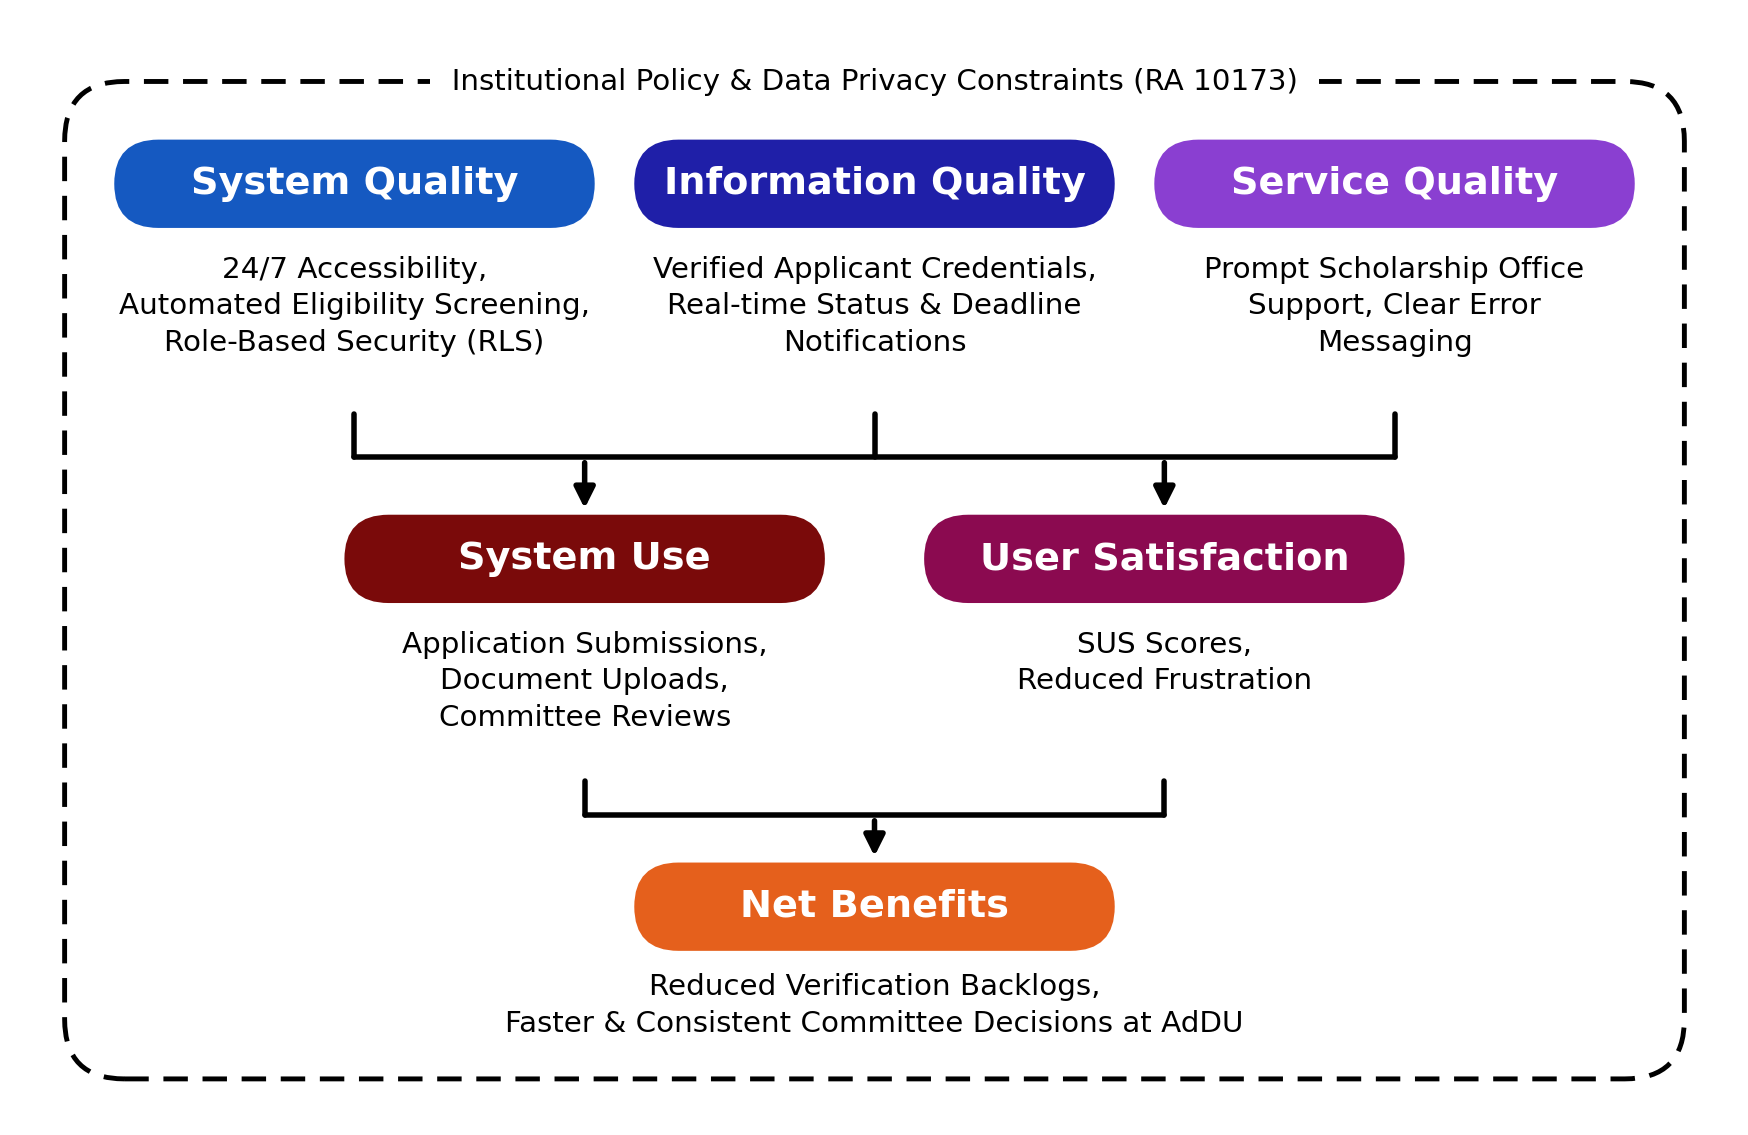
\includegraphics[width=0.85\textwidth]{figure1_issm.png}
  \caption{Adapted Information Systems Success Model for ScholarPath AdDU}
  \label{fig:issm}
\end{figure}

In the context of this study, the foundational dimensions are defined by the platform's technical and informational reliability. System Quality is represented by the portal's 24/7 accessibility, its secure data architecture, and an audit log that traces every status change to a person, each of which responds to the system-architecture gaps documented in the reviewed literature \cite{ref3,ref12,ref14}. Information Quality is reflected in the accuracy of verified applicant data, school-partitioned committee views, and real-time status notifications, addressing the policy desynchronization and information fragmentation identified in \cite{ref16} and \cite{ref36}. Service Quality encompasses the system's responsiveness, including clear correction notices for applicants and prompt workflow support for the University Scholarship Office, informed by the cultural alignment requirements documented in \cite{ref49} and \cite{ref48}. According to the model, high performance in these foundational areas drives user engagement. As applicants, staff, and subcommittee members experience reliable system and information quality, their System Use (e.g., uploading documents, verifying files, recording decisions) and User Satisfaction (measured quantitatively via the System Usability Scale) will increase. Ultimately, this sustained engagement leads to the system's Net Benefits: reduced administrative bottlenecks, fewer applications lost to missing documents, and committee-led decisions that are traceable in an institutional audit. This entire framework operates within the parameters of institutional policy and national data privacy law, with all dimensions of system success governed by the compliance requirements of RA 10173 through the RBAC architecture established in \cite{ref24,ref38}.

\section{Synthesis of RRL and Research Gaps}
\label{sec:synthesis}

The reviewed literature, taken as a whole, establishes a clear progression of scholarship management system capability, from information dissemination \cite{ref12} to submission-enabled portals \cite{ref3,ref14} to multi-function integrated platforms \cite{ref5}, while consistently revealing that no existing implementation resolves the full set of challenges posed by a multi-committee scholarship admission process. The specific gaps motivating ScholarPath AdDU are summarized in Table~\ref{tab:synthesis}, with each gap traced to the reviewed work that documented it.

\begin{table}[htbp]
  \centering
  \small
  \caption{Synthesis of System Gaps and Proposed Design Responses}
  \label{tab:synthesis}
  \begin{tabular}{@{}p{3.0cm}p{5.4cm}p{6.0cm}@{}}
    \toprule
    Reviewed Work & System/Technology Gap Identified & ScholarPath AdDU Design Response \\
    \midrule
    Al-Ayyubi \& Maulana \cite{ref3}; Bagaporo \& Espinosa \cite{ref12} & Portals stop at information dissemination; document submission remains physical and disconnected from the digital workflow. & Two-stage digital submission into the Document Vault, with phase-tagged metadata and versioned corrections under Conditional Revert. \\
    Bilog \cite{ref14} & Unaided eligibility self-assessment drives application errors; rule-based filtering lacked conflict handling. & Phase~1 Pre-qualification flags baseline criteria early; conflicting flags are shown together to staff or the subcommittee, who record the decision. \\
    Kanwal et al. \cite{ref50} & Machine-learned eligibility decisions offer no interpretable audit trail. & Data-Feeding Committee Portal: no module changes an applicant's status without a recorded human actor; every change is written to an audit log. \\
    Amer \cite{ref5} & Single decision body with one flat rule set; multi-unit selection not addressed. & Applicant pool partitioned by school, with five School Scholarship Subcommittee rule sets presented as flags and sort orders. \\
    Mahdi et al. \cite{ref4}; Tunkelang \cite{ref43} & Keyword search fails over multi-attribute records; facets require normalized taxonomy and compound indexing. & Committee filtering with B-Tree and Range compound indexes over school, track, program, status, verification, and score facets; 300\,ms debounce. \\
    Catibog \cite{ref16}; Orgianus et al. \cite{ref36} & Policy desynchronization between published and applied criteria in decentralized systems. & Centralized Supabase/PostgreSQL backend storing the SOP and each school's rule set once; updates propagate to all partitions. \\
    Yoo \& Huang \cite{ref49}; World Bank \cite{ref48} & Misaligned interfaces drive users back to manual processes; mobile-first design is a prerequisite for adoption. & Hybrid web and mobile architecture via Capacitor, from a single Vite codebase. \\
    Halili \cite{ref26}; CHED \cite{ref18} & Limited documentation of RBAC operationalization under RA 10173 in multi-role workflows. & RBAC matrix enforced through PostgreSQL RLS for applicants, staff, interview panels, subcommittees, the Office of Admission, and the System Administrator. \\
    \bottomrule
  \end{tabular}
\end{table}

The convergence of these gaps, namely disconnected document workflows, unaided or automated eligibility decisions without accountability, single-body selection models, policy desynchronization, misaligned interfaces, and undocumented RBAC compliance in Philippine HEI contexts, identifies a distinct and unaddressed design space. No existing implementation in the reviewed literature simultaneously integrates phased digital document submission with structured correction, school-partitioned decision support for multiple selection committees, an audit trail that traces every status change to a person, and proactive notification within a single platform. This gap directly motivates the present study and grounds each architectural decision in ScholarPath AdDU in specific, documented evidence from the reviewed literature.

\chapter{Methodology}
\label{ch:methodology}

This chapter details the systematic procedures, processes, and tools utilized in the design, development, and evaluation of the ScholarPath AdDU system. It outlines the research design, system development methodology, system architecture, data gathering instruments, and statistical tools used for data analysis.

\section{Research Design}
\label{sec:research-design}

This study employs a Developmental Research Design, specifically focusing on System Development. This approach is the most appropriate for IT and Computer Studies capstone projects, as it centers on the structured creation, implementation, and evaluation of a functional software solution to address a specific operational problem. In this context, the design governs the transition of Ateneo de Davao University's (AdDU) paper-based scholarship admission process, as defined in the Standard Procedure for Scholarship Applications (SOP) \cite{ref51}, into a digital, data-feeding workflow that supports the University Scholarship Office and the five School Scholarship Subcommittees. The system requirements are drawn from Key Informant Interviews (KII) with the admissions office and are consolidated in the project's ISO audit preparation report \cite{ref52}. The developmental design is complemented by a descriptive evaluation phase to assess the prototype's usability and functional suitability.

The research design incorporates a comparative usability evaluation to validate the system's impact on processing efficiency. The researchers will administer the Pre-Study Student Problem Validation Survey (Appendix~\ref{app:pre-survey}) to a purposive sample of current or recent AdDU scholarship applicants. This survey measures the perceived time and effort applicants spent on the paper-based process, from reading the scholarship announcement through preparing and physically submitting the SOP application form and its supporting documents. % TODO(L-2): confirm whether Form 230-SCH is the SOP application form.
Once the ScholarPath AdDU prototype is developed, a controlled, task-based usability testing session will be conducted. The perceived time and effort recorded at baseline will then be compared against the corresponding items in the Post-Prototype Perceived Effort Survey (Appendix~\ref{app:post-survey}), which is administered to the same participants immediately following the prototype session. Both instruments use parallel ordinal and Likert-scaled items, enabling direct item-to-item comparisons to determine whether participants perceive the two-stage digital workflow to require less time and effort than the manual process they described at baseline. University Scholarship Office staff and School Scholarship Subcommittee members who complete the staff-side tasks additionally complete the Committee Portal Usefulness Survey (Appendix~\ref{app:committee-survey}). The design and administration of all instruments are detailed in Section~\ref{sec:instruments}.

The comparative evaluation follows a within-subjects design, meaning the same cohort of applicant participants who complete the Pre-Study Survey subsequently participate in the prototype usability testing session. This design is chosen over a between-subjects approach because it eliminates inter-group variability. Each participant serves as their own control, so any observed difference in perceived effort is attributable to the system rather than to individual differences in prior scholarship experience. A sample of 10 to 15 participants is sufficient for this design given that SUS reliability stabilizes at that range \cite{ref42}, and the time-perception comparison uses ordinal scaled data that does not require large-N inferential statistics.

\section{System Development Life Cycle (SDLC)}
\label{sec:sdlc}

To ensure flexibility and iterative improvement, the development of ScholarPath AdDU follows the Agile Development Methodology. Unlike rigid, linear models, Agile allows the development team to adapt to evolving requirements from stakeholders, including the University Scholarship Office, the Office of Admission, and the School Scholarship Subcommittees, through continuous feedback loops between phases. As illustrated in Figure~\ref{fig:sdlc}, the development process is organized into five iterative phases, each building upon the outputs of the last.

\begin{figure}[htbp]
  \centering
  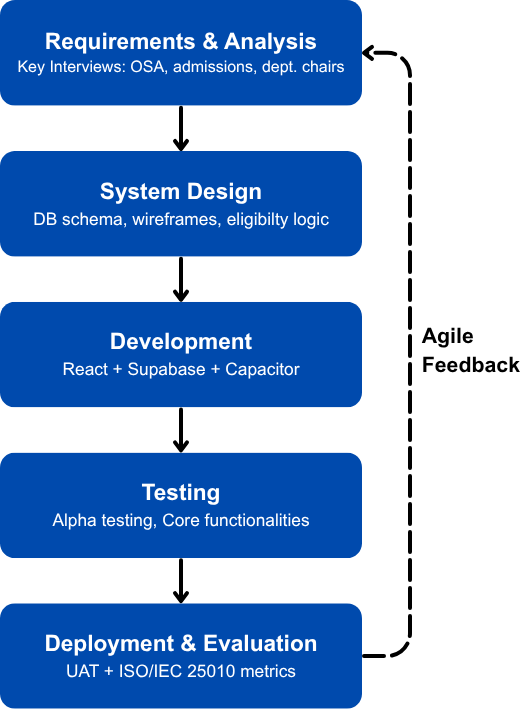
\includegraphics[width=0.8\textwidth]{figure2_p23.png}
  \caption{ScholarPath AdDU Agile SDLC Flowchart}
  \label{fig:sdlc}
\end{figure}

Phase 1: Requirements Gathering. The first phase involves data collection through Key Informant Interviews (KII) with primary stakeholders, including admissions and University Scholarship Office personnel. This phase identifies the eight steps of the SOP \cite{ref51}, the documents required at each step, the selection criteria applied by each School Scholarship Subcommittee, and the points in the process where a person decides an applicant's status. Phase 2: System Design. Drawing from the gathered requirements, this phase produces the architectural blueprint of the system. Deliverables include the relational database schema, User Interface/User Experience (UI/UX) wireframes for applicant, staff, and committee views, and the application status state machine that governs the Application Lifecycle Path. Phase 3: Development. The core programming phase translates design artifacts into a functioning system. Front-end interfaces are built using Vite as the primary build tool, paired with a component-based JavaScript framework (React or Vue) for a reactive, modular UI. Back-end infrastructure, including the PostgreSQL database, secure Document Vault storage, and user authentication, is managed entirely through Supabase. To extend the application to mobile platforms, Capacitor wraps the Vite production build into native Android and iOS packages, enabling cross-platform deployment without maintaining a separate codebase. Phase 4: Testing. Prior to wider release, the system undergoes alpha testing to verify that core functionalities, such as two-stage document uploading, Conditional Revert handling, and human-confirmed status changes, operate without critical errors. Issues surfaced during this phase are documented and fed back into development for resolution before proceeding. Phase 5: Deployment and Evaluation. The functional prototype is deployed to a purposive sample of end-users for User Acceptance Testing (UAT). System quality is then assessed using standardized usability metrics defined by the ISO/IEC 25010 standard, providing quantitative and qualitative data to inform further refinement.

As the feedback loop in Figure~\ref{fig:sdlc} indicates, findings are not terminal; they inform subsequent iterations. The present design is itself the product of one such Adaptation cycle. An earlier prototype automatically assigned students to grants from academic and income data. Following the KII with the admissions office and preparation for an institutional ISO audit \cite{ref52}, that automated matching engine was removed. It was replaced by a data-feeding architecture in which no module assigns, approves, or disapproves an applicant without a recorded human action.

\section{System Architecture and Algorithmic Logic}
\label{sec:architecture}

The architectural decisions underlying ScholarPath AdDU respond to two sources of evidence: the operational requirements documented in the SOP \cite{ref51} and the KII \cite{ref52}, and the gaps identified in the reviewed literature. The choice of a centralized Supabase/PostgreSQL backend was motivated by the policy desynchronization documented in Catibog \cite{ref16} and Orgianus et al. \cite{ref36}, where decentralized systems produced contradictory information that a single canonical database is architecturally positioned to eliminate. The Document Vault and its two-stage submission design directly address the integrated document handling gap identified by both Al-Ayyubi and Maulana \cite{ref3} and Bagaporo and Espinosa \cite{ref12}, whose systems still required physical document submission as a separate, offline step. Bilog's \cite{ref14} finding that unaided self-assessment of eligibility drove application errors motivates Phase~1 Pre-qualification, in which the system flags baseline criteria early and a University Scholarship Office staff member confirms the outcome. Kanwal et al.'s \cite{ref50} acknowledgment that machine-learned eligibility decisions offer no interpretable audit trail motivates the central governance rule of the platform: the system structures, filters, and presents applicant data, and a person makes every decision that changes an applicant's status. The automated notification subsystem responds to the missed-deadline patterns attributable to passive communication channels documented by Catibog \cite{ref16}. Finally, the hybrid mobile-and-web architecture via the Capacitor wrapper was motivated by the World Bank's \cite{ref48} caution that digitization without mobile-first design fails to achieve adoption in Philippine HEI contexts.

\subsection{Scope: Internal Scholarship Tracks}
\label{sec:tracks}

The platform governs the three internal scholarship tracks through which AdDU selects approximately 1,326 applicants per cycle: the Jubilee Scholarship, the Grant-in-Aid (GIA), and the Working Scholars program (Table~\ref{tab:tracks}, Chapter~\ref{ch:introduction}). At registration, each applicant chooses one internal track and up to two degree programs, matching their entrance exam selections. External and government grants, such as those from the Department of Science and Technology (DOST), local government units, and private foundations, are outside the selection process. The university processes their disbursement through financial obligation clearance only after receiving the official beneficiary roster, and the platform treats them as a non-selection pathway.

\subsection{Application Lifecycle Path and Two-Stage Submission}
\label{sec:lifecycle}

The name ScholarPath refers to two structured paths. The Application Lifecycle Path carries an applicant from registration through Phase~1 Pre-qualification, Phase~2 Full Verification, interview scoring, and subcommittee selection, to an award, waitlist, or disapproval outcome. The Academic Trajectory Path then tracks an awarded scholar's academic standing, the completion of service obligations for Working Scholars, and graduation within the contracted degree program. Figure~\ref{fig:lifecycle} presents the end-to-end Application Lifecycle Path.

\begin{figure}[htbp]
  \centering
  % TODO(FIG): replace this placeholder with
  %   \includegraphics[width=\textwidth]{figure_lifecycle.png}
  % drawn to match the ISO audit report's lifecycle diagram (10 steps, 1 loop back).
  \fbox{\parbox{0.92\textwidth}{\centering\small\vspace{0.8em}
    Registration $\rightarrow$ Phase~1 Pre-qualification $\rightarrow$ Phase~2 Full Verification $\rightarrow$ Interview $\rightarrow$ School Subcommittee Selection $\rightarrow$ Release of Results (Office of Admission) $\rightarrow$ Applicant Notified $\rightarrow$ Academic Trajectory Path\\[0.6em]
    Full Verification $\xrightarrow{\text{missing files}}$ Conditional Revert $\xrightarrow{\text{corrected files}}$ Full Verification\\[0.3em]
    Conditional Revert $\xrightarrow{\text{not corrected after 5 days}}$ Lapsed (staff confirm disapproval)\vspace{0.8em}}}
  \caption{Application Lifecycle Path of ScholarPath AdDU}
  \label{fig:lifecycle}
\end{figure}

The revised workflow keeps all eight SOP steps in their original order. It changes only how documents are submitted (step~2) and adds system support for steps~3 to~8, as summarized in Table~\ref{tab:sop-alignment}. % TODO(OPEN-10): will the SOP be formally revised for two-stage submission and Conditional Revert?

\begin{table}[htbp]
  \centering
  \small
  \caption{Alignment of ScholarPath AdDU with the Standard Procedure for Scholarship Applications}
  \label{tab:sop-alignment}
  \begin{tabular}{@{}p{3.6cm}p{6.2cm}p{4.6cm}@{}}
    \toprule
    SOP Step & System Function & Change from SOP \\
    \midrule
    1. Application announcement & Public information page and inquiry form & None \\
    2. Submission of applications & Two-stage digital submission to the Document Vault & Single submission becomes two phases \\
    3. Document verification & University Scholarship Office reviews files in the Document Vault and encodes applicant profiles & None \\ % TODO(OPEN-8): who performs step 3 in practice.
    4. Endorsement to next stage & Qualified applications are released to interview scheduling & None \\
    5. Interview & Interview panel assigned per application records scores and recommendations & Panel composition is configurable \\ % TODO(OPEN-2)
    6. Evaluation and deliberation & School Scholarship Subcommittee reviews data presented by the system and records its decision & None \\
    7. Recommendation and approval & The subcommittee's accepted list is sent to the Office of Admission & System records the handoff \\
    8. Release of results & Office of Admission releases results; applicants are notified only after that release & Notification follows the release event \\
    \bottomrule
  \end{tabular}
\end{table}

Applicants submit documents in two windows (Table~\ref{tab:phases}). In Phase~1 Pre-qualification, the system screens basic eligibility, and pre-qualified applicants receive a provisional go-ahead without submitting a full physical file. In Phase~2 Full Verification, the University Scholarship Office completes verification of the remaining documents before committee review. All credential verification takes place inside the University Scholarship Office; no external or third-party verification service appears in any workflow.

\begin{table}[htbp]
  \centering
  \small
  \caption{Two-Stage Submission Windows and Required Documents}
  \label{tab:phases}
  \begin{tabular}{@{}p{2.6cm}p{2.2cm}p{9.6cm}@{}}
    \toprule
    Phase & Window & Documents \\
    \midrule
    At registration & --- & Application form \\
    Phase 1: Pre-qualification & January to April & Entrance exam result with an ``ACCEPTED'' remark; high school report card (second and third quarter) with a general average of at least 85\%; household income proof; Certificate of Award as Rank~1 or Rank~2 (Jubilee applicants) \\
    Phase 2: Full Verification & May to enrollment & Proof of residence or photographs of residence; recommendation from the homeroom moderator; Certificate of Good Moral Character; BIR Form 2316 or sworn statement of income (GIA and Working Scholars); additional documents configured per cycle, such as a personal essay or an ethnolinguistic group endorsement where applicable \\ % TODO(OPEN-6): residence photos vs. proof; essay and ethnolinguistic endorsement still required?
    \bottomrule
  \end{tabular}
\end{table}

\subsection{Three-Layer Screening and Committee Governance}
\label{sec:governance}

The system structures, filters, and presents applicant data, and people make every decision that changes an applicant's status. Table~\ref{tab:decision-boundary} sets this boundary for each function of the platform. Every status change is written to an audit log that records the acting user, the timestamp, and the prior and new status, so that each decision can be traced to a person during an institutional audit.

\begin{table}[htbp]
  \centering
  \small
  \caption{Decision Boundary Between System Functions and Human Decision-Makers}
  \label{tab:decision-boundary}
  \begin{tabular}{@{}p{3.4cm}p{6.6cm}p{4.4cm}@{}}
    \toprule
    Function & What the System Does & Who Decides \\
    \midrule
    Eligibility screening & Checks baseline criteria (85\% high school average, entrance exam remark, required documents) and flags results & University Scholarship Office staff confirm \\
    Document verification & Stores uploads and shows a checklist per application & University Scholarship Office staff, internally only \\
    Conditional Revert & Sends the notice, runs the 5-day clock, and marks a file ``Lapsed'' & Staff confirm any disapproval \\
    Interview scoring & Records panel scores and recommendations & Interview panel \\
    Selection & Presents applicant data, sorted and filtered by criteria the committee sets & School Scholarship Subcommittee \\
    Waitlist and slot reallocation & Alerts the committee to a vacancy and proposes the next waitlisted candidate & School Scholarship Subcommittee \\
    Track realignment and program transfer & Records the request and checks slot availability & Evaluators and the receiving school \\
    \bottomrule
  \end{tabular}
\end{table}

Evaluation proceeds through three layers. In Layer~1 (General System Verification), the system checks the baseline criteria: an entrance exam result with an ``ACCEPTED'' remark, a high school general average of at least 85\%, and the required documents. An applicant below the baseline, for example with an 84\% average, is not blocked at registration. The application enters a staff review queue, where a University Scholarship Office staff member records a disapproval or waitlist outcome and the applicant receives a notice.

In Layer~2 (Interview Evaluation and Recommendation), interview panels record scores and submit formal recommendations. Following SOP step~5, the interview panel is assigned per application, and panel composition is a configurable setting of each cycle. % TODO(OPEN-2): school-based panels (SOP) vs. Scholarship Director and designated interviewers.
The committee may configure a shortlisting rule that advances a proportion of the interviewed pool, such as the top 50\%, to Layer~3; the system applies no cut unless the committee enables one. % TODO(OPEN-7): is the top-50% cut a formal rule?

In Layer~3 (School Subcommittee Selection), the system partitions applications by degree choice and presents each School Scholarship Subcommittee's data under that school's criteria (Table~\ref{tab:subcommittees}). An applicant whose two program choices fall under different schools appears in both partitions. The system encodes each school's criteria as a rule set that produces flags and sort orders for the committee; it does not produce a selection.

\begin{table}[htbp]
  \centering
  \small
  \caption{School Scholarship Subcommittee Rule Sets}
  \label{tab:subcommittees}
  \begin{tabular}{@{}p{4.2cm}p{3.6cm}p{6.6cm}@{}}
    \toprule
    Subcommittee & Academic Focus & Selection Criteria Presented by the System \\
    \midrule
    School of Nursing (SON) & Nursing and allied health & Zero-conditional policy: conditional entrance exam scores are flagged for rejection; an optional 1-to-10 scoring matrix is available \\
    School of Engineering and Architecture (SEA) & Engineering and architecture programs & Hard cutoffs on entrance exam scores; applicants below the minimum are flagged as not meeting the program requirement regardless of high school rank \\ % TODO(OPEN-4): which school houses Computer Science and IT.
    School of Business and Governance (SBG) & Business and management & Entrance scores combined with financial need tiers and qualitative leadership and potential assessments \\
    School of Education (SOE) & Teacher education & Academic performance weighed alongside commitment to community teaching service \\
    School of Arts and Sciences (SAS) & Humanities, social sciences, and sciences & Academic potential and alignment with university leadership objectives, coordinated across the school's departments \\ % TODO(OPEN-4): four departments with Assistant Deans?
    \bottomrule
  \end{tabular}
\end{table}

The Jubilee Scholarship grant rate is fixed once a Rank~1 or Rank~2 certificate is verified. Program-specific admission minimums remain configurable per school, and when a Jubilee applicant does not meet a school's hard minimum, the system flags the conflict and the subcommittee's recorded decision stands. % TODO(OPEN-3): does the Jubilee guarantee override a hard entrance exam cutoff? TODO(OPEN-9): is the SOP "academic grant" the Jubilee track?

\subsection{Conditional Revert Protocol}
\label{sec:revert}

A missing or illegible document no longer produces an abrupt rejection. Instead, every incomplete file receives five calendar days to be corrected before a staff member decides its outcome:

\begin{enumerate}
  \item A University Scholarship Office staff member finds a missing or illegible document during verification and sets the application status to Conditional Revert.
  \item The platform sends an automated notice that lists each missing or illegible file.
  \item The applicant has five calendar days to upload corrected files. The clock starts at a configurable event, by default the moment the notice is sent. % TODO(OPEN-8): when does the 5-day clock start?
  \item Corrected files return the application to verification.
  \item If nothing arrives within five days, the system marks the file ``Lapsed'' and alerts staff. A University Scholarship Office staff member confirms the disapproval.
\end{enumerate}

Listing~\ref{lst:lifecycle} specifies the application status state machine that enforces this protocol and the governance rule of Section~\ref{sec:governance}. Automated events may only move an application into the Conditional Revert or Lapsed states or raise alerts. Every transition into an outcome state requires a recorded human actor.

\begin{lstlisting}[caption={Pseudocode of the application status state machine with human-confirmation guards},label={lst:lifecycle}]
FUNCTION ChangeStatus(Application, NewStatus, Actor, Reason):
    // Guard 1: outcome states always require a human actor
    IF NewStatus IN {Disapproved, Waitlisted, Awarded, Endorsed} THEN
        RequireHumanActor(Actor)       // reject if Actor is the system
        RequireRole(Actor, AllowedRoles[Application.Status, NewStatus])
    END IF

    // Guard 2: only permitted transitions are accepted
    IF (Application.Status, NewStatus) NOT IN AllowedTransitions THEN
        REJECT "Transition not permitted"
    END IF

    AuditLog.APPEND(Application.ID, Actor, CURRENT_TIMESTAMP,
                    Application.Status, NewStatus, Reason)
    SET Application.Status = NewStatus
    EmitEvent("StatusChanged", Application)
ENDFUNCTION

// Scheduled daily by the Cron worker (system actor)
FUNCTION CheckRevertClocks():
    FOR EACH Application WHERE Status == ConditionalRevert:
        IF CURRENT_DATE > Application.RevertStart + 5 DAYS
           AND Application.HasPendingCorrections THEN
            SET Application.Status = Lapsed    // flag only, not a decision
            AuditLog.APPEND(Application.ID, "system", CURRENT_TIMESTAMP,
                            ConditionalRevert, Lapsed, "Revert window elapsed")
            AlertStaff(Application)            // staff confirm disapproval
        END IF
    ENDFOR
ENDFUNCTION

// Triggered when an awardee declines
FUNCTION OnAwardDeclined(Application):
    FreeSlot(Application.Program, Application.Track)
    Candidate = NextWaitlisted(Application.School, Application.Track)
    AlertSubcommittee(Application.School, ProposedCandidate = Candidate)
    // No award is made until the subcommittee calls ChangeStatus
ENDFUNCTION
\end{lstlisting}

\subsection{Scholar Movement, Track Realignment, and Slot Management}
\label{sec:movement}

The system supports three movement protocols (Table~\ref{tab:movement}). In each, the system records the change and alerts the responsible party immediately, and a person makes the decision.

\begin{table}[htbp]
  \centering
  \small
  \caption{Scholar Movement Protocols}
  \label{tab:movement}
  \begin{tabular}{@{}p{2.6cm}p{4.3cm}p{4.0cm}p{3.5cm}@{}}
    \toprule
    Protocol & Example & System Action & Decision By \\
    \midrule
    Inter-track realignment & A Working Scholar candidate with high financial need and strong academic merit is moved to Grant-in-Aid & Records the change and keeps the history of the applicant's track & Evaluators during screening \\
    External grant program transfer & A DOST awardee must enroll in a specific STEM field, so the applicant moves from Nursing to an engineering program & Checks slot availability in the destination program and records the transfer & Receiving school, subject to slot availability \\
    Waitlist and slot reallocation & A primary awardee declines after receiving an offer from another institution & Frees the slot, alerts the subcommittee, and proposes the next waitlisted candidate & School Scholarship Subcommittee confirms; the candidate is notified after confirmation \\
    \bottomrule
  \end{tabular}
\end{table}

\subsection{Committee Filtering and Backend Indexing Strategy}
\label{sec:filtering}

To let the University Scholarship Office and each School Scholarship Subcommittee review approximately 1,326 applications per cycle without manual collation, the Data-Feeding Committee Portal exposes applicant records through intersecting filters (e.g., ``School = SEA'' + ``Track = GIA'' + ``Verification Status = Complete''). The available facets are school, track, program choice, lifecycle status, verification status, interview score, and screening flags. The sort order and filter criteria are set by the committee, not by the system. Indexing Strategy for Real-Time Retrieval: to ensure real-time rendering, the Supabase backend uses compound indexing, pre-sorting records on frequently queried combinations instead of scanning the entire table for every query.

\begin{itemize}
  \item B-Tree Indexes are applied to exact-match categorical fields (e.g., \texttt{School\_Code}, \texttt{Track}, and \texttt{Status}).
  \item Range Indexes are applied to continuous numerical and temporal fields (e.g., \texttt{HS\_Average}, \texttt{Interview\_Score}, and \texttt{Revert\_Start}).
  \item Client-Side Caching and Debouncing: The frontend interface uses asynchronous JavaScript (Fetch) combined with an input debounce of 300 milliseconds, so the database is queried only after the user finishes selecting facets, reducing server load and preventing interface stutter.
\end{itemize}

\subsection{System Architecture and Cloud Infrastructure}
\label{sec:cloud}

To resolve the operational bottlenecks caused by the physical submission of dense paperwork, ScholarPath AdDU employs a secure, cloud-based architecture. The integration of the database, storage, and communication services is mapped in Figure~\ref{fig:architecture}.

\begin{figure}[htbp]
  \centering
  % TODO(FIG): redraw figure4_architecture.png -- relabel the client apps as
  % "Applicant/Scholar App" and "Committee Portal"; add an Audit Log store in
  % the backend layer; keep no external verification service.
  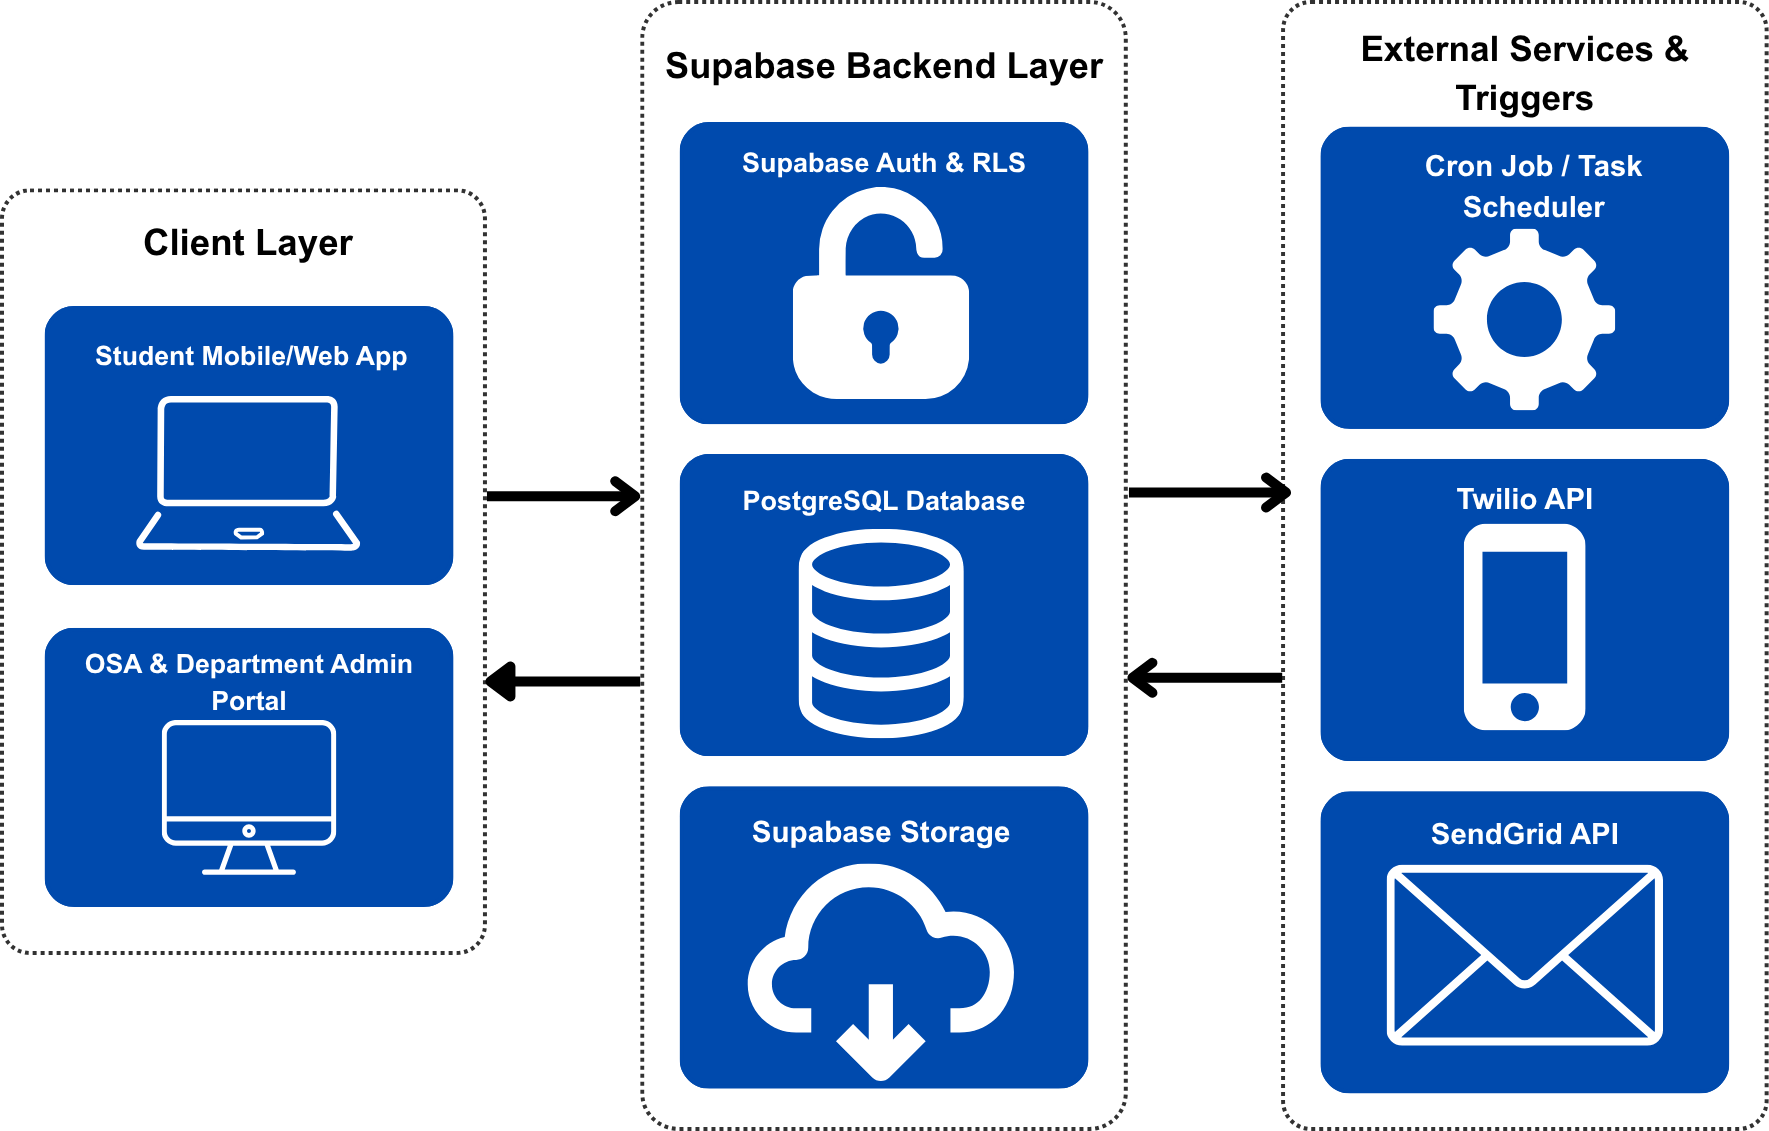
\includegraphics[width=0.9\textwidth]{figure4_architecture.png}
  \caption{High-Level System Architecture of ScholarPath AdDU}
  \label{fig:architecture}
\end{figure}

Technical Stack and Storage: The system is built on a three-layer technical stack selected for its cohesion and rapid prototyping capabilities. At the client layer, Vite serves as the frontend build tool, paired with a component-based JavaScript framework (React or Vue), and provides two interfaces: the applicant and scholar application, and the Data-Feeding Committee Portal used by University Scholarship Office staff, interview panels, School Scholarship Subcommittees, and the Office of Admission. For cross-platform mobile deployment, Capacitor wraps the same Vite production build into native Android and iOS applications. At the backend layer, Supabase serves as the core Backend-as-a-Service (BaaS) infrastructure, providing a hosted PostgreSQL relational database for system state, metadata, and the audit log; Supabase Storage for large object files (the Document Vault); and Supabase Auth integrated natively with Row Level Security (RLS) policies.

Metadata Tagging and Phase-Aware Storage: When an applicant uploads a document, the physical file is stored exactly once in a dedicated Supabase Storage bucket under a unique, secure path. A Documents table records the file's metadata (e.g., \texttt{ApplicantID}, \texttt{DocumentType}, \texttt{Phase}, \texttt{UploadTimestamp}, \texttt{Verification\_Status}, and \texttt{Storage\_Path}), and the Applications table links to it by foreign key. A corrected file uploaded during a Conditional Revert is stored as a new version linked to the same requirement, preserving the history of what was submitted and when.

Document Verification Workflow: Every uploaded document, including proof-of-income documents such as BIR Form 2316 or a sworn statement, is automatically assigned a verification status of Pending. A University Scholarship Office staff member reviews the document through the Committee Portal and manually updates its status to Verified, or sets the application to Conditional Revert if the document is missing or illegible. Applications with Pending or unresolved documents cannot be endorsed to interview scheduling. All verification is performed internally by the University Scholarship Office; the platform integrates with no external verification service.

\subsection{Role-Based Access Control (RBAC) and Data Privacy Compliance}
\label{sec:rbac}

Because the ScholarPath AdDU platform processes highly sensitive economic and academic data, its architecture is governed by the Philippine Data Privacy Act of 2012 (RA 10173). Encryption and Row Level Security (RLS): All data in transit is secured using Transport Layer Security (TLS). Access to sensitive data at rest, in both database tables and Supabase Storage buckets, is restricted using RLS policies, so access controls are enforced directly at the database level regardless of how the frontend is accessed. RBAC Permissions Matrix: To enforce the principle of least privilege, users are assigned distinct privileges based on their role within the university, mapped directly to database RLS policies (Table~\ref{tab:rbac}).

\begin{table}[htbp]
  \centering
  \small
  \caption{ScholarPath AdDU Role-Based Access Control (RBAC) Matrix}
  \label{tab:rbac}
  \begin{tabular}{@{}p{3.2cm}p{5.2cm}p{6.0cm}@{}}
    \toprule
    User Role & Data Access Privileges & Core System Actions \\
    \midrule
    Applicant / Scholar & Read/write, self only & Register, choose a track and up to two programs, upload Phase~1 and Phase~2 documents, respond to Conditional Revert notices, view status and Academic Trajectory Path \\
    University Scholarship Office staff & Read/write, all applications & Verify documents, set Conditional Revert, confirm Lapsed disapprovals, record Layer~1 outcomes, endorse applications to interview, broadcast announcements \\
    Interview Panel & Read, assigned applications only; write, own scores & Record interview scores and recommendations \\
    School Scholarship Subcommittee & Read, own school's partition; write, own decisions & Filter and sort applicants, record selection decisions, confirm waitlist reallocations, send the accepted list to the Office of Admission \\
    Office of Admission & Read, accepted lists & Release results, which triggers applicant notifications \\
    System Administrator & Configuration only & Configure cycle windows, rule sets, and roles; no authority over applicant status \\
    \bottomrule
  \end{tabular}
\end{table}

\subsection{Automated Notification Subsystem}
\label{sec:notifications}

The absence of proactive alerts frequently results in missed submission windows and uncorrected files. ScholarPath AdDU integrates an automated, multi-channel notification subsystem that delivers deadline reminders, correction notices, and status updates via SMS and email. Third-Party API Integration: The SendGrid API formats and dispatches detailed email notifications, and the Twilio SMS API pushes brief, time-sensitive text messages to the applicant's registered mobile device. These services deliver messages only; they take no part in verification or decisions. Automated Trigger Logic and Edge Functions: The notification engine is driven by scheduled tasks (Cron jobs) and Supabase Edge Functions evaluating three conditions:

\begin{enumerate}
  \item Deadline Proximity: A scheduled worker queries the database daily. If the current date is within a predefined threshold (e.g., three days) of the close of the Phase~1 or Phase~2 window and the applicant has outstanding documents, an Edge Function sends a reminder via Twilio.
  \item Conditional Revert Clock: When staff set an application to Conditional Revert, an Edge Function sends the correction notice listing each missing or illegible file, followed by reminders within the five-day window. When the window elapses, the Lapsed flag triggers an alert to University Scholarship Office staff rather than a message to the applicant.
  \item Status Mutation: When a human actor commits a status change, a database webhook triggers an Edge Function. Selection outcomes are withheld from applicants until the Office of Admission records the release of results, after which the award, waitlist, or disapproval notice is sent via SendGrid. A waitlisted candidate is notified of a reallocated slot only after the subcommittee confirms the reallocation. % TODO(OPEN-8): notification timing after the Office of Admission release.
\end{enumerate}

\section{Testing \& Evaluation Procedures: ISO/IEC 25010 Task-Based Usability Protocol}
\label{sec:testing}

To assess the functional suitability and usability of the ScholarPath AdDU system, the study employs a mixed-method evaluation approach. This methodology combines task-based observational testing with a standardized System Usability Scale (SUS) questionnaire, administered to a purposive sample of approximately 10 to 15 end-users. The sample will consist of current or recent scholarship applicants, University Scholarship Office staff, and School Scholarship Subcommittee members, to guarantee coverage of the system's multi-role interfaces.

\subsection{Step-by-Step Testing Procedure}
\label{sec:procedure}

The evaluation will be conducted in a controlled environment following a standardized script to prevent researcher bias. The procedure is outlined as follows:

\begin{enumerate}
  \item Briefing and Consent: Participants are introduced to the system's purpose. The facilitator explicitly states that the system is being tested, not the user, and secures informed consent.
  \item Task Execution: Participants complete the tasks for their role. The facilitator observes silently without offering assistance unless a critical failure occurs.
  \begin{itemize}
    \item Task 1: Applicant Registration (applicants): The user creates an account, completes the application form, and selects one internal track and up to two degree programs.
    \item Task 2: Two-Stage Document Submission (applicants): The user uploads the Phase~1 documents, then the Phase~2 documents, and responds to a Conditional Revert notice by uploading a corrected file.
    \item Task 3: Verification and Conditional Revert (University Scholarship Office staff): The user verifies an application's documents, sets a Conditional Revert on an application with a missing file, and confirms the disapproval of a Lapsed application.
    \item Task 4: Committee Review and Reallocation (School Scholarship Subcommittee members): The user filters the school's partition, records a selection decision, and confirms a proposed waitlist reallocation after an awardee declines.
  \end{itemize}
  \item Observational Data Collection: During task execution, the facilitator records the usability metrics detailed in Section~\ref{sec:analysis}.
  \item Post-Session Instruments: Immediately after completing the tasks, participants complete the standardized 10-item System Usability Scale (SUS) questionnaire first, capturing their holistic impression before any comparative framing is introduced. Applicant participants then complete the Post-Prototype Perceived Effort Survey (Appendix~\ref{app:post-survey}); staff and subcommittee participants complete the Committee Portal Usefulness Survey (Appendix~\ref{app:committee-survey}). These instruments are not to be conflated: the SUS measures general interface usability, while the role-specific surveys generate the comparative and perception data used to answer Research Questions 1 through 3.
  \item Debriefing: A brief, semi-structured exit interview is conducted to gather qualitative feedback on any frustrations or difficulties encountered.
\end{enumerate}

\subsection{Data Analysis and Statistical Tools}
\label{sec:analysis}

To objectively quantify the system's performance and user satisfaction, the following metrics and statistical tools will be utilized:

\begin{itemize}
  \item Quantitative Observational Metrics:
  \begin{itemize}
    \item Time-on-Task: Measured in seconds, this records the duration a user takes to successfully complete each designated task.
    \item Error Rates: Calculated as the number of misclicks, failed uploads, or incorrect navigation paths taken per task, as well as the overall percentage of users who fail to complete a task independently.
    \item Notification Delivery Success Rate: Measured during Tasks 3 and 4, this metric records the percentage of triggered notification events (the Conditional Revert notice sent when a staff participant sets the status, and the outcome notice sent after a simulated Office of Admission release) that result in a successfully dispatched notification to the applicant's registered contact channel within the testing session. The facilitator confirms delivery on the designated applicant-side test device. The metric is computed as: (Number of Successfully Delivered Notifications / Total Triggered Notification Events) $\times$ 100. A delivery success rate of 100\% is the target threshold, given the controlled, low-concurrency testing environment.
    \item Trigger-to-Delivery Latency: Recorded in seconds, this measures the elapsed time between the moment a staff participant commits a status change (the event trigger) and the moment the corresponding notification is confirmed as received on the applicant-side test device. Mean latency across all triggered events in the session is computed and reported, operationalizing the performance efficiency of the notification subsystem as distinct from overall system response time.
  \end{itemize}
  \item System Usability Scale (SUS) Analysis:
  \begin{itemize}
    \item The SUS provides a validated instrument for measuring participants' subjective perceived usability of the platform. Responses are gathered on a standard 5-point Likert scale across 10 items, with alternating positive and negative phrasing to reduce response bias. Raw SUS scores, ranging from 0 to 100, will be analyzed using descriptive statistics. The Mean will be calculated to determine the average perceived usability score across the purposive sample. To contextualize the resulting mean SUS score, the study will apply the adjective rating scale validated by Bangor et al. \cite{ref13}: scores of 85 and above are classified as Excellent, 71--84 as Good, 50--70 as OK, and below 50 as indicative of usability failure requiring significant redesign. A target mean SUS score of 71 or higher (the Good threshold) is set as the minimum benchmark for the prototype to be considered functionally acceptable for its intended user base. The Standard Deviation will measure the variance in scores, indicating the degree of consensus among participants. The SUS addresses Research Question 4 specifically and is analytically distinct from the comparative instruments described below.
  \end{itemize}
  \item Functional Correctness Evaluation (Lifecycle Test Case Matrix):
  \begin{itemize}
    \item To assess whether the application status state machine (Listing~\ref{lst:lifecycle}) executes the Application Lifecycle Path correctly and never changes an applicant's status without a recorded human actor, corresponding to the Functional Correctness sub-characteristic of ISO/IEC 25010 (Table~\ref{tab:iso25010}), the study employs a structured test case matrix administered separately from the user-facing usability session (Table~\ref{tab:lifecycle-tests}). For each case, the expected system output is documented prior to test execution; the actual output is then recorded and compared. A match constitutes a pass; any discrepancy constitutes a failure and is logged for root cause analysis. The Functional Correctness score is computed as: (Number of Passing Test Cases / Total Test Cases) $\times$ 100. A pass rate of 100\% on the human-confirmation cases (TC-05, TC-07, TC-12, TC-13, and TC-16) is set as the non-negotiable threshold, because a status change without a recorded human actor is the highest-risk failure mode of the platform.
  \end{itemize}
  \item Pre/Post Comparative Survey Analysis:
  \begin{itemize}
    \item The Pre-Study Student Problem Validation Survey (Appendix~\ref{app:pre-survey}) and the Post-Prototype Perceived Effort Survey (Appendix~\ref{app:post-survey}) together constitute the comparative data collection instruments for Research Questions 1 and 3. Because both instruments use structurally parallel items with identical scale anchors, their data is analyzed through direct item-level comparisons using descriptive statistics.
    \item For Component 1 of both instruments (the ordinal time-estimation scale), the distribution of responses across the five ordinal ranges will be tabulated for both conditions. The modal response category and the direction of shift will be reported to address RQ1.
    \item For Component 2 of both instruments (the six-item perceived effort Likert grid), the Mean score per sub-task item will be calculated for both conditions and presented in a side-by-side comparison table. A decrease in mean score from pre- to post-prototype indicates a perceived reduction in effort for that application stage. Sub-task items 1 through 5 inform RQ1, and sub-task item 6 (deadline and correction tracking) informs RQ3.
    \item For Component 3 of both instruments, frequency distributions will be used for the categorical items concerning incomplete-document history and missed-deadline history (RQ3). The proportion of participants who reported an application delayed or rejected because of a missing or illegible document will be compared against the proportion who indicated that the Conditional Revert notice would let them correct such a file in time. Similarly, the proportion who reported missing deadlines will be compared against post-prototype responses on the notification subsystem's perceived effectiveness.
    \item For Component 4 of the post-prototype instrument (the overall comparative perception item), a frequency distribution of responses across the five-point scale will be reported as a summary indicator of the system's perceived overall impact.
  \end{itemize}
  \item Committee Portal Usefulness Analysis: Responses to the Committee Portal Usefulness Survey (Appendix~\ref{app:committee-survey}) will be summarized as item means and standard deviations to address RQ2(b).
  \item Qualitative Data Analysis (Thematic Analysis): The qualitative feedback gathered during the post-task semi-structured exit interviews will be processed using thematic analysis. The researchers will transcribe participant comments and categorize them into recurring themes (e.g., ``Navigation Friction,'' ``Terminology Confusion,'' or ``Positive Interface Feedback''). These themes will provide contextual explanations for the quantitative error rates and guide the final iterative refinements of the system's user interface prior to deployment.
\end{itemize}

\begin{longtable}{@{}p{1.2cm}p{6.6cm}p{6.6cm}@{}}
  \caption{Lifecycle Test Case Matrix}\label{tab:lifecycle-tests}\\
  \toprule
  ID & Test Profile & Expected System Output \\
  \midrule
  \endfirsthead
  \toprule
  ID & Test Profile & Expected System Output \\
  \midrule
  \endhead
  \bottomrule
  \endfoot
  TC-01 & High school average exactly 85\%, entrance exam ``ACCEPTED'', all Phase~1 documents & No baseline flag; application proceeds to Phase~2 \\
  TC-02 & High school average 84\% & Registration not blocked; application enters the staff review queue with a below-baseline flag; no status change until staff act \\
  TC-03 & Entrance exam result without an ``ACCEPTED'' remark & Baseline flag raised; application enters the staff review queue \\
  TC-04 & Jubilee applicant without a Rank~1 or Rank~2 certificate & Missing-document flag on the Jubilee requirement; application cannot be endorsed \\
  TC-05 & Phase~2 document missing; staff set Conditional Revert & Status becomes Conditional Revert; notice lists the missing file; audit log records the staff actor \\
  TC-06 & Corrected file uploaded on day~5 of the Revert window & Application returns to verification; no Lapsed flag \\
  TC-07 & No correction by day~6 & Status becomes Lapsed and staff are alerted; status does not become Disapproved until a staff member confirms \\
  TC-08 & SON applicant with a conditional entrance exam score & SON rule set flags the applicant; no selection is recorded by the system \\
  TC-09 & SEA applicant below the entrance exam cutoff & SEA rule set flags the applicant as not meeting the program minimum; decision remains with the subcommittee \\
  TC-10 & Applicant whose two program choices belong to different schools & Application appears in both schools' partitions \\
  TC-11 & Subcommittee records an award before the Office of Admission release & Status is recorded; no notification reaches the applicant until the release event \\
  TC-12 & Awardee declines the offer & Slot freed; subcommittee alerted with a proposed waitlisted candidate; no award to the candidate until the subcommittee confirms \\
  TC-13 & Attempt by a system process to set Disapproved, Waitlisted, or Awarded & Transition rejected by the human-actor guard \\
  TC-14 & Inter-track realignment from Working Scholars to GIA & Track changed by an evaluator; prior track retained in history and audit log \\
  TC-15 & Subcommittee member attempts to view another school's partition & Access denied by RLS \\
  TC-16 & Any completed test case & Every status change in the audit log carries an actor, timestamp, prior status, and new status \\
\end{longtable}

\subsection{Pre-Study, Post-Prototype, and Committee Survey Instruments}
\label{sec:instruments}

To operationalize the within-subjects comparative design described in Section~\ref{sec:research-design}, this study employs two structurally paired applicant instruments administered at distinct phases of the research process, together with a single-administration staff instrument. The Pre-Study Student Problem Validation Survey (Appendix~\ref{app:pre-survey}) is administered prior to system exposure to establish baseline data on the perceived burden of the existing paper-based process. The Post-Prototype Perceived Effort Survey (Appendix~\ref{app:post-survey}) is administered immediately following the task-based usability testing session using an identical scale structure. Together, these instruments generate the comparative data required to address Research Questions 1 and 3. Because each participant's pre-study responses serve as their own baseline, any observed reduction in perceived effort can be attributed to the system's features rather than to differences in prior scholarship experience. Both instruments use scaled and categorical response formats rather than open recall of specific durations, acknowledging that the manual application process unfolds over days or weeks and is not conducive to precise time measurement.

Pre-Study Student Problem Validation Survey (Appendix~\ref{app:pre-survey}). The pre-study instrument is administered to a purposive sample of current or recent AdDU scholarship applicants prior to any system exposure. It is organized into three components. Component 1: Perceived Time-on-Process asks respondents to estimate the total duration of their end-to-end manual application experience, from reading the scholarship announcement through physically submitting the application form and supporting documents, using five ordinal ranges: less than 1 day, 1--3 days, 4--7 days, 1--2 weeks, and more than 2 weeks. This item establishes the time-burden baseline for RQ1. Post-prototype time estimates are derived from a controlled testing session and may not reflect the duration of the process in real-world deployment, where document readiness, network conditions, and platform familiarity may produce different results. Component 2: Perceived Effort Scale applies a five-point Likert format (1 = Very Easy, 5 = Very Difficult) to six application sub-tasks: (1) understanding which scholarship track to apply for and what it requires; (2) determining whether they met the baseline requirements, such as the high school average, entrance exam result, rank certificate, and income documents, before submitting; (3) gathering, printing, and preparing the required physical documents; (4) physically submitting the completed application package; (5) tracking the status of the application after submission; and (6) keeping track of submission deadlines and requests for missing documents. Sub-tasks 1 through 5 establish the effort baseline for RQ1, and sub-task 6 establishes the deadline and correction baseline for RQ3. Component 3: Document and Deadline History uses categorical items to establish behavioral baselines for RQ3. Respondents are asked whether an application of theirs was ever delayed or rejected because of a missing or illegible document, and how often; and whether they ever missed a scholarship application deadline, and for what primary reason.

Post-Prototype Perceived Effort Survey (Appendix~\ref{app:post-survey}). The post-prototype instrument is administered to the same participants after the SUS questionnaire. Its structural mirroring of the pre-study instrument is deliberate: because both instruments use identical Likert anchors, ordinal ranges, and sub-task categories, their corresponding items can be compared directly. Component 1 presents the same five ordinal time-estimation ranges. Component 2 presents the same six sub-tasks, reworded to reflect ScholarPath AdDU's features: track and program selection at registration; understanding the Phase~1 Pre-qualification result; uploading documents through the Document Vault; submitting the application digitally; tracking status through the applicant dashboard; and staying aware of deadlines and correction requests through the notification subsystem. Component 3: System Feature Effectiveness asks whether the Conditional Revert notice would help participants correct a missing or illegible document before their application lapses, and how far the automated notifications would help them remain aware of upcoming deadlines. Component 4: Overall Comparative Perception asks participants to characterize the total effort required by ScholarPath AdDU relative to the paper-based process on a five-point scale. An optional open-ended item closes the instrument.

Committee Portal Usefulness Survey (Appendix~\ref{app:committee-survey}). University Scholarship Office staff and School Scholarship Subcommittee members who complete Tasks 3 and 4 rate, on a five-point agreement scale, whether the Committee Portal presents the information they need to decide, whether the school partition and filters reduce manual collation, whether the audit log makes decisions traceable, and whether they retain full control over every status decision. These items address RQ2(b).

\section{Ethical Considerations}
\label{sec:ethics}

Because the usability testing of ScholarPath AdDU involves human participants and the simulated input of sensitive socioeconomic data, the evaluation phase is strictly governed by established research ethics and the Philippine Data Privacy Act of 2012 (RA 10173). The following ethical protocols will be implemented throughout the testing phase:

\begin{itemize}
  \item Informed Consent and Voluntary Participation: Prior to any system interaction, all participants will be provided with an informed consent form detailing the purpose of the study, the specific tasks required, and the estimated time commitment. Because scholarship applicants may be incoming first-year students under 18 years of age, participants who are minors will additionally require the written consent of a parent or guardian together with their own assent. Participation is strictly voluntary, and participants maintain the right to withdraw from the testing session at any point without penalty or need for justification. % TODO(L-4): confirm minor-consent requirements with the ethics adviser.
  \item Data Anonymization and Privacy: During task execution, participants will be explicitly instructed to use provided mock data or pseudonymized profiles rather than their actual household income, grades, or documents. This ensures that no genuine sensitive information is exposed or recorded during the evaluation.
  \item Confidentiality and Secure Data Disposal: All observational metrics, survey responses (Appendices~\ref{app:pre-survey} to~\ref{app:committee-survey}), and SUS questionnaire responses will be kept strictly confidential. Data will be aggregated so that no single metric or quote can be traced back to an individual participant. Upon the successful defense and final submission of the capstone project, all test accounts, mock databases, and physical consent forms utilized during the evaluation phase will be permanently and securely deleted.
\end{itemize}

\chapter{Theoretical Background}
\label{ch:theory}

\section{Introduction}
\label{sec:theory-intro}

The design and implementation of ScholarPath AdDU is grounded in nine established theoretical frameworks drawn from computer science, information science, and software engineering. Together, these theories provide formal justification for every major architectural decision, from database structure and document management to security, user experience, and development methodology. This chapter situates each theory within the overarching Information Systems Success Model \cite{ref20} adopted in Chapter~\ref{ch:rrl}. Relational Database Theory and Metadata-Driven Document Management underpin System Quality by ensuring structural integrity and storage efficiency. Information Foraging Theory and Event-Driven Architecture support Information and Service Quality through improved discoverability of applicant data and proactive communication. Rule-Based Screening Theory, bounded by a human-in-the-loop decision rule, explains how the platform turns the SOP and the five school rule sets into flags that inform, but never make, committee decisions. Finally, Cloud Infrastructure Theory, RBAC, Empirical Process Control, and the HCI/ISO 25010 framework collectively ensure scalability, legal compliance, iterative development, and empirically validated usability.

\section{Relational Database Theory and Normalization}
\label{sec:relational}

Consolidating applicant academic records, household financial documents, interview scores, five school rule sets, and an audit log of human decisions into a consistent repository requires a rigorous structural foundation. Relational Database Theory, specifically the normalization principles formalized by Codd \cite{ref17}, provides this foundation by organizing data into interconnected two-dimensional tables governed by first-order predicate logic. Within the DeLone and McLean \cite{ref20} framework, a normalized 3NF schema is the foundational enabler of System Quality, specifically the sub-dimension of data integrity, as it eliminates the inconsistencies that would otherwise corrupt the data presented to committees.

\subsection{The Relational Model and Anomaly Prevention}
\label{sec:anomalies}

Codd \cite{ref17} defined normalization as the systematic process of organizing relations to reduce redundancy and prevent modification anomalies. In the AdDU context, three anomaly types directly threaten the integrity of an unnormalized scholarship admission database. Table~\ref{tab:anomalies} outlines each anomaly and its resolution within ScholarPath AdDU.

\begin{table}[htbp]
  \centering
  \small
  \caption{Database Anomalies and Their Resolution in ScholarPath AdDU}
  \label{tab:anomalies}
  \begin{tabular}{@{}p{2.4cm}p{5.2cm}p{6.8cm}@{}}
    \toprule
    Anomaly Type & Definition & Resolution in ScholarPath AdDU \\
    \midrule
    Insertion Anomaly & Facts cannot be recorded because they lack a required primary key from another entity. & School rule sets and track definitions are stored independently of applications, so a subcommittee's criteria for a new cycle can be configured before any applicant registers. \\
    Update Anomaly & A single logical fact recorded across multiple rows creates contradictions when updates are partially executed. & Each baseline threshold, phase window, and school criterion exists in one canonical row; an update propagates to every partition and concurrent committee query. \\
    Deletion Anomaly & Deleting one record unintentionally destroys data representing an entirely different, independent fact. & Withdrawing an application does not remove its audit log entries or the school's rule set, which are stored in independent relations. \\
    \bottomrule
  \end{tabular}
\end{table}

\subsection{Progression Through Normal Forms}
\label{sec:normal-forms}

The ScholarPath AdDU schema adheres to the Third Normal Form (3NF), progressing through Codd's sequential requirements. First Normal Form (1NF) mandates atomic, scalar values with no repeating groups; prerequisite documents such as the application form, report card, and BIR Form 2316 are therefore stored as discrete, queryable records rather than comma-separated strings. Second Normal Form (2NF) eliminates partial dependencies, ensuring school and track details are stored independently of application records. Third Normal Form (3NF) eliminates transitive dependencies, ensuring, as Kent \cite{ref32} summarizes, that every non-key attribute provides ``a fact about the key, the whole key, and nothing but the key.'' Adhering to 3NF guarantees that any update to a configured parameter, such as a revised baseline average or an extended Phase~2 window, propagates from a single authoritative record to all related queries.

\section{Centralized Information Systems and Cloud Infrastructure Theory}
\label{sec:cloud-theory}

The decision to deploy ScholarPath AdDU as a single unified web platform, rather than distributing applicant data across the files of five school subcommittees, is grounded in centralized IT infrastructure theory \cite{ref34}. Centralized infrastructure consolidates computing resources and data into one managed environment, enabling uniform policy enforcement and the elimination of data silos that cause policy desynchronization across departments \cite{ref41}. By hosting the entire SOP-aligned Application Lifecycle Path on a single Supabase backend, changes to submission windows or school criteria are immediately reflected for all users. Modern cloud platforms mitigate the traditional risk of centralization, a single point of failure, through hardware virtualization and physical redundancy. Mell and Grance \cite{ref34} define cloud computing as on-demand access to a shared pool of configurable computing resources characterized by rapid elasticity and measured service. For ScholarPath AdDU, Supabase's managed PostgreSQL infrastructure provides high availability, and the platform's audit log of every status change supports both compliance with the Philippine Data Privacy Act of 2012 (RA 10173) and the traceability expected in institutional quality audits \cite{ref52}. % TODO(OPEN-1): name the ISO standard once confirmed.
In the IS Success Model, centralized cloud infrastructure directly supports System Quality through 24/7 availability and Service Quality through uniform, institution-wide policy enforcement.

\section{Metadata-Driven Document Management}
\label{sec:metadata}

Manual, paper-based document workflows create severe operational bottlenecks for the University Scholarship Office, which must receive and check a complete physical file from every applicant. ScholarPath AdDU resolves this through metadata-driven document management, which decouples physical file storage from logical document associations \cite{ref25}. Table~\ref{tab:storage} contrasts traditional hierarchical storage with the metadata-driven approach.

\begin{table}[htbp]
  \centering
  \small
  \caption{Traditional Hierarchical Storage versus Metadata-Driven Architecture}
  \label{tab:storage}
  \begin{tabular}{@{}p{2.8cm}p{5.4cm}p{6.2cm}@{}}
    \toprule
    Feature & Traditional Hierarchical Storage & Metadata-Driven Architecture \\
    \midrule
    Location Strategy & Files are locked into a rigid folder path. & Files are stored in a flat virtual pool; organization is determined dynamically by relational metadata tags. \\
    Submission Phases & A single complete file must be assembled and submitted at once. & Each document is tagged with its submission phase, so Phase~1 and Phase~2 documents accumulate against one application. \\
    Corrections & A replaced page overwrites or is filed separately from the original. & A corrected upload during a Conditional Revert is stored as a new version of the same requirement, preserving the submission history. \\
    Retrieval Mechanism & Staff navigate a folder hierarchy to locate files. & Staff query by document type, phase, upload date, or verification status. \\
    \bottomrule
  \end{tabular}
\end{table}

ScholarPath AdDU operationalizes this theory as the Document Vault. When an applicant uploads a prerequisite file, such as a report card or BIR Form 2316, it is stored exactly once in a Supabase Storage bucket and assigned a unique URI. The Applications table references that file through foreign keys, and its metadata records the submission phase and verification status. University Scholarship Office staff can therefore query and verify documents through metadata tags rather than folder hierarchies.

\section{Rule-Based Screening and Human-in-the-Loop Decision Support}
\label{sec:rule-screening}

Rule-Based Expert Systems (RBS) theory represents domain expertise as conditional IF-THEN logic \cite{ref15}. ScholarPath AdDU applies this theory in a deliberately bounded way. The rules encode the SOP baseline and the five School Scholarship Subcommittee rule sets, but their conclusions are flags, sort orders, and alerts, never verdicts on an applicant. The decision that changes an applicant's status is always made and recorded by a person. This boundary answers the interpretability concern that Kanwal et al. \cite{ref50} raise about automated scholarship eligibility decisions, and it is the architectural expression of the institutional directive that no algorithm selects scholars \cite{ref52}. % TODO(L-6): add team-supplied decision-support / human-oversight sources as ref53+.
In the DeLone and McLean \cite{ref20} model, rule-based screening supports Information Quality, specifically the completeness and relevance of the data a committee sees, while the human decision rule supports the accountability of the Net Benefits the system produces.

\subsection{Knowledge Representation and the Inference Engine}
\label{sec:knowledge}

Buchanan and Duda \cite{ref15} describe expert systems as consisting of three interdependent components: a Knowledge Base of facts and IF-THEN rules, a Working Memory storing the current input state, and an Inference Engine that applies rules to derive conclusions via the logical principle of modus ponens. In ScholarPath AdDU, the Knowledge Base is the SOP baseline (an entrance exam ``ACCEPTED'' remark, a high school general average of at least 85\%, and the required documents) together with the five school rule sets; the Working Memory is an application's verified data at a given lifecycle stage; and the Inference Engine applies a forward-chaining strategy from those data to a set of screening flags. The conclusions of the engine are routed to a staff review queue or displayed in the Committee Portal, where a person acts on them.

\subsection{Rule Precedence and Committee Resolution}
\label{sec:precedence}

A core design challenge in rule-based systems is conflict resolution: determining behavior when multiple rules apply to the same data state. In ScholarPath AdDU, conflicts arise when a track rule and a school rule point in different directions. For example, a certified Rank~1 graduate qualifies for the fixed Jubilee grant rate, while the SEA rule set applies a hard entrance exam cutoff to the same applicant's program choice. The platform does not resolve such conflicts automatically. It raises both flags, shows them together to the School Scholarship Subcommittee, and records the subcommittee's decision. % TODO(OPEN-3): Jubilee guarantee vs. school hard cutoff.
Table~\ref{tab:conflict} maps the conflict resolution strategies to their system context.

\begin{table}[htbp]
  \centering
  \small
  \caption{Rule Conflict Handling in ScholarPath AdDU Screening}
  \label{tab:conflict}
  \begin{tabular}{@{}p{3.0cm}p{5.0cm}p{6.4cm}@{}}
    \toprule
    Strategy & Theoretical Definition & ScholarPath AdDU Implementation \\
    \midrule
    Specificity Priority & Rules with more specific conditions are evaluated before general rules. & School-specific rules, such as the SON zero-conditional policy, are evaluated and displayed alongside the general SOP baseline flags. \\
    Flag, Do Not Fire & Conflicting conclusions are surfaced rather than acted upon. & When a track rule and a school rule conflict, both flags are shown to the subcommittee; no status change occurs until a member records a decision. \\
    Human Resolution & A designated authority resolves conflicts that rules cannot. & The School Scholarship Subcommittee's recorded decision stands and is written to the audit log with the acting member and timestamp. \\
    \bottomrule
  \end{tabular}
\end{table}

\section{Information Foraging Theory and Committee Filtering}
\label{sec:ift}

The cognitive processes through which users navigate complex digital environments are formalized by Information Foraging Theory (IFT), developed by Pirolli and Card \cite{ref37} at PARC. IFT applies optimal foraging theory from evolutionary ecology to model how users maximize the rate of information gain while minimizing cognitive cost. IFT rests on three core constructs: Information Patches (localized clusters of related content within an interface), Information Diet (the specific subset of sources a user pursues to satisfy a goal), and Information Scent (the user's cognitive estimate of how likely a given path is to yield relevant results). When perceived scent drops below a threshold, users abandon the current patch and navigate elsewhere \cite{ref37}. In the AdDU context, a subcommittee member facing an undifferentiated list of approximately 1,326 applications experiences weak information scent and high foraging cost. ScholarPath AdDU addresses this by partitioning applications by school, so each subcommittee begins in its own patch, and by exposing the underlying metadata as filters, such as track, program choice, verification status, and interview score, that the member intersects to refine the patch \cite{ref4,ref43}. Backend compound indexing and a 300-millisecond client-side debounce ensure fast query response, preserving the low temporal cost critical to effective information foraging.

\section{Event-Driven Architecture for Asynchronous Notification}
\label{sec:eda}

Missed submission windows and uncorrected files are attributable in part to passive, manual communication channels. ScholarPath AdDU addresses this through Event-Driven Architecture (EDA), which shifts the notification system from a synchronous request-response model to an asynchronous, event-triggered one \cite{ref28}. EDA is built around the production, detection, and consumption of events, defined as significant changes in system state, and operates on the principle of loose coupling, where components interact independently with no awareness of each other's internal logic. By adopting EDA, the notification subsystem operates without blocking the main application server. Table~\ref{tab:eda} maps the event triggers to their corresponding EDA components.

\begin{table}[htbp]
  \centering
  \small
  \caption{Event-Driven Architecture Trigger Mapping for the Automated Notification Subsystem}
  \label{tab:eda}
  \begin{tabular}{@{}p{2.2cm}p{4.0cm}p{4.0cm}p{4.2cm}@{}}
    \toprule
    EDA Component & Temporal Trigger (Deadlines and Revert Clock) & Transactional Trigger (Human Status Change) & Transactional Trigger (Release and Vacancy) \\
    \midrule
    Event Producer & Scheduled Cron job checking phase windows and five-day Revert clocks daily & Staff or subcommittee member committing a status change & Office of Admission recording the release of results; an awardee declining an offer \\
    Event Router & Database logic identifying applications near a deadline or past the Revert window & Database webhook detecting the change upon commit & Database webhook detecting the release or the freed slot \\
    Event Consumer & Edge Function sending an SMS reminder via Twilio, or flagging the file Lapsed and alerting staff & Edge Function sending a Conditional Revert notice via SendGrid and Twilio & Edge Function sending outcome notices to applicants, or alerting the subcommittee with a proposed waitlisted candidate \\
    \bottomrule
  \end{tabular}
\end{table}

This decoupled architecture ensures that third-party API latency, inherent in calls to Twilio and SendGrid, is absorbed entirely by the Edge Function layer, allowing the core web server to scale efficiently under concurrent load. It also enforces the ordering required by the SOP: an applicant's outcome notice is produced only by the release event of the Office of Admission, never by the subcommittee's decision itself.

\section{Role-Based Access Control and Data Privacy}
\label{sec:rbac-theory}

Scholarship admission systems process highly sensitive personal and socioeconomic data, necessitating rigorous access control. ScholarPath AdDU implements the NIST Role-Based Access Control (RBAC) model, formalized by Ferraiolo and Kuhn \cite{ref24} and standardized by NIST in 2004. RBAC replaced error-prone, per-user Access Control Lists (ACLs) with a tripartite structure: Users are assigned Roles representing their organizational function, and Permissions are attached exclusively to those Roles \cite{ref38}. This structure inherently enforces two foundational security principles: the Principle of Least Privilege, which limits access to the minimum required for each user's duties, and Separation of Duties, which distributes critical workflows across roles to prevent unilateral fraud or error. Separation of Duties is especially visible in ScholarPath AdDU: University Scholarship Office staff verify documents, interview panels score, School Scholarship Subcommittees select, and the Office of Admission releases results, so no single role carries an application from submission to award. RBAC is also the direct mechanism by which the platform complies with RA 10173. Applicants hold self-access only; staff hold access to all applications for verification; interview panels see only their assigned applications; each subcommittee sees only its own school's partition; and the System Administrator configures the platform without authority over any applicant's status (Table~\ref{tab:rbac}). These boundaries are enforced at the database engine level through PostgreSQL Row Level Security (RLS) policies. Within the IS Success Model, RBAC is the mechanism by which the platform satisfies the Service Quality dimension, specifically the assurance sub-dimension.

\section{Empirical Process Control Theory in Agile Development}
\label{sec:agile-theory}

The development of ScholarPath AdDU is governed by Empirical Process Control theory, the foundational pillar of Agile methodology \cite{ref39}. Unlike the Waterfall model, which assumes complete upfront specification of all requirements, empirical process control acknowledges that complex software systems operate in volatile, ambiguous environments where requirements emerge through iterative stakeholder interaction. The theory rests on three interdependent pillars \cite{ref39}: Transparency, requiring that all development progress and system artifacts be visible and understood by both developers and stakeholders; Inspection, requiring frequent examination of the system against standard metrics to detect variances; and Adaptation, requiring immediate process adjustment when inspection reveals unacceptable deviation. The five school rule sets and the SOP contain procedural details that cannot be fully specified before development begins, several of which remain under confirmation with the University Scholarship Office. The development of ScholarPath AdDU has already exercised all three pillars. Key Informant Interviews with the admissions office served as Inspection, revealing that an earlier automated matching design conflicted with institutional governance, and the redesign into a data-feeding architecture was the resulting Adaptation \cite{ref52}. The Agile SDLC described in Chapter~\ref{ch:methodology} continues this cycle through alpha testing and User Acceptance Testing (UAT). In the context of the IS Success Model, empirical process control supports System Quality by enabling continuous verification that the system's functional logic aligns with stakeholder requirements. Hoda et al. \cite{ref27} conducted a systematic mapping of agile practices across 1,540 studies, confirming that transparency, iterative inspection, and stakeholder-driven adaptation remain the dominant predictors of project success in environments characterized by evolving or partially specified requirements, conditions that describe AdDU's scholarship admission procedures.

\section{Human-Computer Interaction and the ISO/IEC 25010 Model}
\label{sec:hci}

While robust backend architecture ensures computational reliability, the practical success of an information system is ultimately determined by user adoption. The interface design and formal evaluation of ScholarPath AdDU are therefore guided by Human-Computer Interaction (HCI) theory and the ISO/IEC 25010:2023 Software Quality Evaluation standard \cite{ref23,ref31}. HCI focuses on designing interactive computing systems that align with users' cognitive capacities and actual workflows \cite{ref23}. For applicants, the legacy process of assembling a complete physical file, submitting it in person, and waiting without status updates imposes unnecessary cognitive and logistical overhead. ScholarPath AdDU alleviates this through an applicant dashboard showing the current lifecycle stage, outstanding documents, and correction requests, and through a mobile-responsive architecture enabling uploads from any device. For staff and subcommittee members, the Committee Portal replaces manual collation with partitioned, filterable views.

The ISO/IEC 25010:2023 SQuaRE standard provides the formal evaluation framework, defining product quality across eight measurable characteristics. The ScholarPath AdDU prototype assessment operationalizes two dimensions, Functional Suitability and Performance Efficiency, as detailed in Table~\ref{tab:iso25010}.

\begin{table}[htbp]
  \centering
  \small
  \caption{ISO/IEC 25010:2023 Evaluation Dimensions for ScholarPath AdDU}
  \label{tab:iso25010}
  \begin{tabular}{@{}p{2.8cm}p{3.2cm}p{8.4cm}@{}}
    \toprule
    Characteristic & Sub-Characteristic & Evaluation Metric for ScholarPath AdDU \\
    \midrule
    Functional Suitability & Functional Completeness & Verifies that the system covers all designated tasks without omission: applicant registration, two-stage document submission and Conditional Revert response, staff verification, and committee review and reallocation. \\
    & Functional Correctness & Assesses, through the Lifecycle Test Case Matrix, whether status transitions follow the Application Lifecycle Path and whether every status change carries a recorded human actor. \\
    & Functional Appropriateness & Examines whether the applicant dashboard and Committee Portal facilitate rapid task completion within the University Scholarship Office's operational context. \\
    Performance Efficiency & Time Behavior & Measures system response times, document upload speed, committee filtering latency, and notification trigger-to-delivery latency. \\
    & Resource Utilization & Monitors cloud resource use, ensuring compound indexing minimizes database load during peak submission windows. \\
    \bottomrule
  \end{tabular}
\end{table}

Evaluation will be conducted through task-based usability testing with a purposive sample of 10 to 15 participants, complemented by post-session instruments: the standardized 10-item System Usability Scale (SUS), which addresses Research Question 4; the Post-Prototype Perceived Effort Survey (Appendix~\ref{app:post-survey}), compared against the pre-study baseline (Appendix~\ref{app:pre-survey}) to address Research Questions 1 and 3; and the Committee Portal Usefulness Survey (Appendix~\ref{app:committee-survey}), which addresses Research Question 2(b). By measuring error rates and time-on-task against the ISO/IEC 25010 dimensions, and by comparing pre- and post-prototype perceived effort for document submission, correction, status tracking, and deadline awareness, ScholarPath AdDU will be empirically validated as a functional, efficient, and user-centric solution to AdDU's scholarship admission bottlenecks.


%----- References ------------------------------------------------------
\printbibliography[heading=bibintoc]

%----- Appendices ------------------------------------------------------
\appendix
\chapter{Internal Financial Aid Pipelines Listed at AdDU}
\label{app:pipelines}

The following table reproduces the inventory of the internal scholarship tracks consolidated by ScholarPath AdDU.

% Internal scholarship tracks inventory (revised manuscript, Appendix A).
\begin{longtable}{@{}r p{7.0cm} l p{5.0cm}@{}}
\caption{Internal Financial Aid Pipelines Listed at AdDU}\label{tab:appendix-a}\\
\toprule
\# & Scholarship Name & Category & Source URL / Reference \\
\midrule
\endfirsthead
\toprule
\# & Scholarship Name & Category & Source URL / Reference \\
\midrule
\endhead
\bottomrule
\endfoot
1 & Jubilee Scholarship Fund (Valedictorian \& Salutatorian) & Internal Track & \url{https://www.addu.edu.ph/list-of-scholarship-grants/} \\
2 & Grant-In-Aid (GIA) Fund & Internal Track & \url{https://www.addu.edu.ph/scholarships-and-financial-aid-for-college/} \\
3 & Student Assistant (SA) Program / Working Scholars & Internal Track & \url{https://www.addu.edu.ph/student-assistants/} \\
\end{longtable}

\chapter{Pre-Study Student Problem Validation Survey}
\label{app:pre-survey}

% TODO(L-3): this version assumes the survey has NOT yet been administered.
% If it has, restore the administered version from git history and keep only
% the Section 3.4.3 remapping.

\section*{Screening}

Question 1: Have you ever applied for an Ateneo de Davao University scholarship (Jubilee Scholarship, Grant-in-Aid, or Working Scholars) using the paper-based application process?

\begin{itemize}
  \item Question Type: Multiple Choice
  \item Options:
  \begin{itemize}
    \item Yes (Continue to next section)
    \item No (Submit form; not a target respondent)
  \end{itemize}
\end{itemize}

\section*{Component 1: Perceived Time-on-Process}

Please recall your most recent experience applying for an AdDU scholarship using the paper-based process.

Question 2: How much total time did you spend on the entire application process? (This includes reading the announcement, gathering requirements, completing the application form, and physically submitting the documents.)

\begin{itemize}
  \item Question Type: Multiple Choice
  \item Options:
  \begin{itemize}
    \item Less than 1 day
    \item 1 -- 3 days
    \item 4 -- 7 days
    \item 1 -- 2 weeks
    \item More than 2 weeks
  \end{itemize}
\end{itemize}

\section*{Component 2: Perceived Effort Scale}

Question 3: On a scale of 1 to 5, please rate how easy or difficult it was to complete the following application steps.

\begin{itemize}
  \item Question Type: Likert Grid (5-point scale)
  \item Scale Columns: 1 --- Very Easy; 2 --- Easy; 3 --- Neutral; 4 --- Difficult; 5 --- Very Difficult
  \item Row Sub-tasks:
  \begin{enumerate}
    \item Understanding which scholarship track to apply for and what it required.
    \item Determining whether you met the baseline requirements (such as the high school average, entrance exam result, rank certificate, and income documents) before submitting.
    \item Gathering, printing, and preparing the required physical documents.
    \item Physically submitting the completed application package.
    \item Tracking the status of your application after submission.
    \item Keeping track of submission deadlines and requests for missing documents.
  \end{enumerate}
\end{itemize}

\section*{Component 3: Document and Deadline History}

Question 4: Was your scholarship application ever delayed or rejected because a document was missing or illegible?

\begin{itemize}
  \item Question Type: Multiple Choice
  \item Options:
  \begin{itemize}
    \item Yes
    \item No
    \item I am not sure
  \end{itemize}
\end{itemize}

Question 5: (Displayed only if ``Yes'' is selected in Question 4.) Approximately how many times did this occur?

\begin{itemize}
  \item Question Type: Multiple Choice
  \item Options:
  \begin{itemize}
    \item Once
    \item 2 -- 3 times
    \item 4 or more times
  \end{itemize}
\end{itemize}

Question 6: Have you ever missed a scholarship application deadline while using the paper-based process?

\begin{itemize}
  \item Question Type: Multiple Choice
  \item Options:
  \begin{itemize}
    \item Yes
    \item No
  \end{itemize}
\end{itemize}

Question 7: (Displayed only if ``Yes'' is selected in Question 6.) What was the primary reason you missed that deadline?

\begin{itemize}
  \item Question Type: Multiple Choice
  \item Options:
  \begin{itemize}
    \item I was unaware that the deadline existed or had passed
    \item I did not have enough time to prepare the required physical documents
    \item I did not know that a document was missing until it was too late
    \item Other (Please specify)
  \end{itemize}
\end{itemize}

\chapter{Post-Prototype Perceived Effort Survey}
\label{app:post-survey}

\section*{Component 1: Perceived Time-on-Process}

Based on your experience using the ScholarPath AdDU prototype during the testing session, please answer the following.

Question 1: How much total time do you estimate the digital scholarship application process through ScholarPath AdDU would require? (This includes registering, choosing a track and programs, uploading Phase~1 and Phase~2 documents to the Document Vault, and correcting any missing documents.)

\begin{itemize}
  \item Question Type: Multiple Choice
  \item Options:
  \begin{itemize}
    \item Less than 1 day
    \item 1 -- 3 days
    \item 4 -- 7 days
    \item 1 -- 2 weeks
    \item More than 2 weeks
  \end{itemize}
\end{itemize}

\section*{Component 2: Perceived Effort Scale}

Please use the same scale you applied in the pre-study survey for direct comparison.

Question 2: On a scale of 1 to 5, please rate how easy or difficult it was to complete each of the following steps using ScholarPath AdDU.

\begin{itemize}
  \item Question Type: Likert Grid (5-point scale)
  \item Scale Columns: 1 --- Very Easy; 2 --- Easy; 3 --- Neutral; 4 --- Difficult; 5 --- Very Difficult
  \item Row Sub-tasks:
  \begin{enumerate}
    \item Choosing a scholarship track and up to two degree programs at registration.
    \item Understanding your Phase~1 Pre-qualification result and what was still required.
    \item Uploading and managing the required documents through the Document Vault.
    \item Submitting your application digitally through the platform.
    \item Tracking the status of your application through the applicant dashboard.
    \item Staying aware of submission deadlines and correction requests through the notification system.
  \end{enumerate}
\end{itemize}

\section*{Component 3: System Feature Effectiveness}

Question 3: Do you believe the Conditional Revert notice, which lists each missing or illegible document and gives you five calendar days to upload a correction, would help you complete your application before it lapses?

\begin{itemize}
  \item Question Type: Multiple Choice
  \item Options:
  \begin{itemize}
    \item Yes, it would let me correct my documents in time
    \item Partially; it would help, but I might still miss the window
    \item No, I do not think it would make a difference
    \item Unsure
  \end{itemize}
\end{itemize}

Question 4: The automated deadline and correction notifications in ScholarPath AdDU would make it easier to stay aware of upcoming application deadlines.

\begin{itemize}
  \item Question Type: Likert Scale
  \item Options: 5 --- Strongly Agree; 4 --- Agree; 3 --- Neutral; 2 --- Disagree; 1 --- Strongly Disagree
\end{itemize}

\section*{Component 4: Overall Comparative Perception}

Question 5: Compared to the paper-based scholarship application process, how would you characterize the overall effort required to complete a scholarship application using ScholarPath AdDU?

\begin{itemize}
  \item Question Type: Multiple Choice
  \item Options:
  \begin{itemize}
    \item Much Easier
    \item Somewhat Easier
    \item About the Same
    \item Somewhat Harder
    \item Much Harder
  \end{itemize}
\end{itemize}

Question 6 (Optional): Which specific feature of ScholarPath AdDU most reduced the difficulty of the scholarship application process for you? Please describe briefly.

\begin{itemize}
  \item Question Type: Short Answer (Open-ended)
\end{itemize}

\chapter{Pre-Study Administrative Process Validation Survey}
\label{app:pre-admin-survey}

This survey is for university personnel involved in processing applications for AdDU's internal scholarship tracks. Please answer based on the most recent application cycle handled through the manual, paper-based process. Please complete this survey before seeing or testing ScholarPath AdDU.

Question 1: What is your role in the scholarship application process?

\begin{itemize}
  \item Question Type: Multiple Choice
  \item Options:
  \begin{itemize}
    \item Office head or supervisor
    \item Staff (screening and document verification)
    \item School Scholarship Subcommittee member
    \item Other (please specify) Component 1: Perceived Processing Time Question 2: On average, how much staff time does it take to process a single scholarship application, from receiving it to marking it ready for interview or subcommittee evaluation? (Include screening and document verification; exclude the interview itself.)
  \end{itemize}
  \item Question Type: Multiple Choice
  \item Options:
  \begin{itemize}
    \item Less than 15 minutes
    \item 15 -- 30 minutes
    \item 31 -- 60 minutes
    \item 1 -- 2 hours
    \item More than 2 hours Question 3: How long does one full application cycle take, from the opening of applications to the release of results?
  \end{itemize}
  \item Question Type: Multiple Choice
  \item Options:
  \begin{itemize}
    \item Less than 2 weeks
    \item 2 -- 4 weeks
    \item 1 -- 2 months
    \item 2 -- 3 months
    \item More than 3 months Component 2: Perceived Effort Scale Question 4: On a scale of 1 to 5, please rate how easy or difficult each of the following tasks is for your office under the manual process.
  \end{itemize}
  \item Question Type: Likert Grid (5-point scale)
  \item Scale Columns:
  \begin{itemize}
    \item 1 - Very Easy
    \item 2 - Easy
    \item 3 - Neutral
    \item 4 - Difficult
    \item 5 - Very Difficult
  \end{itemize}
  \item Row Sub-tasks: 1. Receiving, sorting, and filing incoming paper applications. 2. Checking whether each applicant meets the baseline requirements (high school average, entrance exam result, household income) of the chosen track. 3. Verifying submitted documents against official report cards and income documents. 4. Requesting missing or corrected documents from applicants and tracking whether they were submitted. 5. Collating evaluation results from interview panels and the five School Scholarship Subcommittees. 6. Identifying who made or approved a specific status change or decision on an application. 7. Informing applicants of their application status, correction requests, and deadlines. Component 3: Processing Issues History Question 5: In a typical application cycle, how often does each of the following happen?
  \item Question Type: Likert Grid (5-point frequency scale)
  \item Scale Columns:
  \begin{itemize}
    \item 1 - Never
    \item 2 - Rarely
    \item 3 - Sometimes
    \item 4 - Often
    \item 5 - Very Often
  \end{itemize}
  \item Row Items: 1. A full application file is processed even though the applicant does not meet the baseline requirements. 2. An application is incomplete or contains an illegible document. 3. An applicant does not submit requested missing or corrected documents before the deadline. 4. An applicant misses a submission deadline. 5. Interview or subcommittee results have to be re-encoded or collated manually. 6. It is unclear who made or approved a decision on an application. 7. Applicants contact the office to ask about the status of their application. Question 6 (Optional): Which part of the manual process creates the most work for your office? Please describe briefly.
  \item Question Type: Short Answer (Open-ended)
\end{itemize}

\chapter{Post-Prototype Administrative Evaluation Survey}
\label{app:post-admin-survey}

Please answer the following based on your experience using the Unified Admin Dashboard of ScholarPath AdDU during the testing session. The same scales as in the pre-study survey are used so that your answers can be compared directly.

Component 1: Perceived Processing Time

Question 1: Using ScholarPath AdDU, how much staff time do you estimate it would take to process a single scholarship application, from receiving it to marking it ready for interview or subcommittee evaluation?

\begin{itemize}
  \item Question Type: Multiple Choice
  \item Options:
  \begin{itemize}
    \item Less than 15 minutes
    \item 15 -- 30 minutes
    \item 31 -- 60 minutes
    \item 1 -- 2 hours
    \item More than 2 hours Question 2: Using ScholarPath AdDU, how long do you estimate one full application cycle would take, from the opening of applications to the release of results?
  \end{itemize}
  \item Question Type: Multiple Choice
  \item Options:
  \begin{itemize}
    \item Less than 2 weeks
    \item 2 -- 4 weeks
    \item 1 -- 2 months
    \item 2 -- 3 months
    \item More than 3 months Component 2: Perceived Effort Scale Question 3: On a scale of 1 to 5, please rate how easy or difficult each of the following tasks would be for your office using ScholarPath AdDU.
  \end{itemize}
  \item Question Type: Likert Grid (5-point scale)
  \item Scale Columns:
  \begin{itemize}
    \item 1 - Very Easy
    \item 2 - Easy
    \item 3 - Neutral
    \item 4 - Difficult
    \item 5 - Very Difficult
  \end{itemize}
  \item Row Sub-tasks: 1. Receiving and organizing incoming applications through the Unified Admin Dashboard. 2. Checking baseline requirements using the flags produced by the Smart Eligibility Checker. 3. Verifying uploaded documents in the Document Vault. 4. Requesting corrected documents through the Conditional Revert window and tracking re-uploads. 5. Viewing interview and subcommittee results in a single dashboard. 6. Identifying who made a specific status change using the system's audit log. 7. Informing applicants of status changes and deadlines through automated SMS and email notifications. Component 3: Perceived Usefulness of the Unified Admin Dashboard Question 4: Please indicate how much you agree with each statement. (Items adapted from the Perceived Usefulness scale of Davis~\cite{ref51}.)
  \item Question Type: Likert Grid (5-point scale)
  \item Scale Columns:
  \begin{itemize}
    \item 5 - Strongly Agree
    \item 4 - Agree
    \item 3 - Neutral
    \item 2 - Disagree
    \item 1 - Strongly Disagree
  \end{itemize}
  \item Row Items: 1. Using the Unified Admin Dashboard would enable our office to process scholarship applications more quickly. 2. Using the Unified Admin Dashboard would improve the accuracy of applicant screening and document verification. 3. Using the Unified Admin Dashboard would reduce the manual work of collating interview and subcommittee results. 4. Using the Unified Admin Dashboard would make it easier to trace who made each decision on an application. 5. Using the Unified Admin Dashboard would make our office's scholarship work easier overall. 6. I would find the Unified Admin Dashboard useful in our office's scholarship application process. Component 4: System Feature Effectiveness Question 5: Please indicate how much you agree with each statement.
  \item Question Type: Likert Grid (5-point scale)
  \item Scale Columns:
  \begin{itemize}
    \item 5 - Strongly Agree
    \item 4 - Agree
    \item 3 - Neutral
    \item 2 - Disagree
    \item 1 - Strongly Disagree
  \end{itemize}
  \item Row Items: 1. The Smart Eligibility Checker flags would reduce the time staff spend on applicants who do not meet baseline requirements. 2. The 5-calendar-day Conditional Revert window would reduce the number of incomplete applications. 3. The automated SMS and email notifications would reduce the number of applicants who miss deadlines or correction requests. 4. The automated notifications would reduce the number of status inquiries the office receives. 5. The role-based access in the dashboard, where each office sees only the data it needs, is appropriate for the office's data privacy obligations under RA~10173. Component 5: Overall Comparative Perception Question 6: Compared to the current manual process, how would you characterize the overall effort required for your office to process scholarship applications using ScholarPath AdDU?
  \item Question Type: Multiple Choice
  \item Options:
  \begin{itemize}
    \item Much Easier
    \item Somewhat Easier
    \item About the Same
    \item Somewhat Harder
    \item Much Harder Component 6: Open-Ended Feedback Question 7 (Optional): Which feature of ScholarPath AdDU would most reduce your office's workload? Please describe briefly.
  \end{itemize}
  \item Question Type: Short Answer (Open-ended) Question 8 (Optional): What would need to change or be added before your office could adopt ScholarPath AdDU for an actual application cycle?
  \item Question Type: Short Answer (Open-ended)
\end{itemize}


\end{document}
